\documentclass[12pt]{exam}

\newcommand{\Solutions}{1} 
\newcommand{\SetNumber}{1} % can set this variable to zero here it gets updated automatically later
\newcommand{\Version}{2} 
\newcommand{\TestName}{}
\newcommand{\TB}{Exam 2}
\newcommand{\Exam}{2}

% LOAD PACKAGES
\usepackage{amsmath} % allows for align env and other things
\usepackage{amssymb} % 
\usepackage{mathtools} % allows for single apostrophe
\usepackage{enumitem} % allows for alpha lettering in enumerated lists
\usepackage{lastpage}
\usepackage{array} % for table alignments 
\usepackage{comment} 

% TIKZ DIAGRAMS (IF NEEDED)
\usepackage{color}
\usepackage{tikz}  \usetikzlibrary{arrows, automata} 
\usetikzlibrary{calc} 

% SUBSPACES AND ORTHOGONALITY
\newcommand{\Perp}{^{\perp}}
\newcommand{\Row}{\text{Row}}
\newcommand{\Col}{\text{Col}}
\newcommand{\Nul}{\text{Null}}
\newcommand{\Null}{\text{Null}}
\newcommand{\proj}{\text{proj}}
\newcommand{\Span}{\text{Span}}
\newcommand{\Rank}{\text{rank}}
\newcommand{\Dim}{\text{dim}}

% ADJUST MARGINS
\usepackage[tmargin=2.2in,bmargin=1.75in]{geometry}
\geometry{margin=0.75in}

% COLORS FOR DIAGRAMS IN SOLUTIONS
\definecolor{DarkBlue}{rgb}{0.0,0.2,0.4} % 

% HEADERS AND FOOTERS
\pagestyle{headandfoot}
\runningfooter{}{}{}
\runningheader{\textit{\TestName}}{}{\textit{Page \thepage \ of \pageref{LastPage}} }
% \headheight 42pt % distance from top of page to top of header
% \headsep 12pt % space between header and top of body

\newcommand{\ID}{Fill in the blanks with a dark pen or pencil. 
Using only capital letters print your \\ first name: \framebox{\strut\hspace{4.2cm}}, last name: \framebox{\strut\hspace{4.2cm}}, the remaining digits \\[2pt] of your GTID:  \framebox{\strut $9$}\framebox{\strut $0$}\framebox{\strut\hspace{0.19cm}}\framebox{\strut\hspace{0.19cm}}\framebox{\strut\hspace{0.19cm}}\framebox{\strut\hspace{0.19cm}}\framebox{\strut\hspace{0.19cm}}\framebox{\strut\hspace{0.19cm}}\framebox{\strut\hspace{0.19cm}}, the high school you attend: \framebox{\strut\hspace{5.2cm}}.}

% ADJUST FIRST LINE IN PARAGRAPH INDENTATION 
\setlength\parindent{0pt}

% FONT FORMAT
\renewcommand*\rmdefault{lmss} % change font to lat mod ss


% AUGMENTED MATRIX
\newenvironment{amatrix}[1]{%
  \left(\begin{array}{@{}*{#1}{c}|c@{}}
}{%
  \end{array}\right)
}

% ~ ~ ~ ~ ~ ~ ~ ~ ~ ~ ~ ~ ~ ~ ~ ~ ~ ~ ~ ~ ~ ~ ~ ~ ~ ~ ~ 
% CUSTOMIZED EMPHASIS
\newcommand{\Emph}[1]{{\color{DarkBlue}\textbf{#1}}} 

% \usepackage{titlesec}
% % \usepackage{lipsum}
% \titleformat{\section}
%   {\normalfont}{\thesection}{0em}{}

% \titleformat{\section}[wrap]
% {\normalfont}
% {\thesection.}{0.5em}{}

% --------------------------------------------------------------------
\begin{document}
\input{Cover/CoverPage}
\foreach \i in {1,...,8} {
\renewcommand{\Version}{\i} 

\ifnum \Version=0 \renewcommand{\TestName}{Version 0} \fi
\ifnum \Version=1 \renewcommand{\TestName}{Year 1 MATH 1554 Exam 2 Sample A} \fi
\ifnum \Version=2 \renewcommand{\TestName}{Year 1 MATH 1554 Exam 2 Sample B} \fi
\ifnum \Version=3 \renewcommand{\TestName}{Year 1 MATH 1554 Exam 2 Sample C} \fi
\ifnum \Version=4 \renewcommand{\TestName}{Year 1 MATH 1554 Exam 2 Sample D} \fi
\ifnum \Version=5 \renewcommand{\TestName}{Year 1 MATH 1554 Exam 2 Sample E} \fi
\ifnum \Version=6 \renewcommand{\TestName}{Year 1 MATH 1554 Exam 2 Sample F} \fi
\ifnum \Version=7 \renewcommand{\TestName}{Year 1 MATH 1554 Exam 2 Sample G} \fi
\ifnum \Version=8 \renewcommand{\TestName}{Year 1 MATH 1554 Exam 2 Sample H} \fi
\ifnum \Version=20 \renewcommand{\TestName}{Year 1 MATH 1554 Exam 2 Sample I} \fi


% TITLE
\begin{center}
\ifnum \Solutions=1 {\Large {\color{DarkBlue}\textit{Solutions}}\\[6pt]}\fi
\ifnum \Solutions=1 
    {\color{DarkBlue} Answers below each question.\\ Don't hesitate to ask questions on the course forum and/or office hours about any of the solutions.\\[12pt] }
\fi
{\Large \TestName}
\end{center}

    \input{202408/Exam2/Q}
\newpage


% \ifnum \SetNumber=1
%     % \ifnum \Solutions=1 \newpage \fi
%     % \question[2] Fill in the blanks. You do not need to show your work. 
%     % \begin{parts}
%     %     \input{202408/Exam2/Q4a}
%     %     \part

\ifnum \Version=1
    If $A$ is $2 \times 3$ and is in RREF, and $\vec x = \begin{pmatrix} 2&3&-1\end{pmatrix}^T$ spans $\Null A$, then $A=\begin{pmatrix} a_1 & a_2 & a_3 \\ a_4 & a_5 & a_6 \end{pmatrix} $ where 
    $a_1 = \framebox{\strut\hspace{1.0cm}}$, 
    $a_2 = \framebox{\strut\hspace{1.0cm}}$, 
    $a_3 = \framebox{\strut\hspace{1.0cm}}$, 
    $a_4 = \framebox{\strut\hspace{1.0cm}}$,
    $a_5 = \framebox{\strut\hspace{1.0cm}}$,
    $a_6 = \framebox{\strut\hspace{1.0cm}}$.

    \ifnum \Solutions=1 {\color{DarkBlue} \textit{Solutions.} 

    If $x$ spans $\Null A$ then $A$ has two pivots. Since $A$ must also be in RREF we can set $a_1=a_5=1$ and $a_2=a_4 = 0$. So far we have
    $$A = \begin{pmatrix} 1&0&a_3\\0&1&a_6\end{pmatrix}$$
    But $A\vec x = \vec 0$, so 
    \begin{align}
        A\vec x = \begin{pmatrix} 1&0&a_3\\0&1&a_6\end{pmatrix}\begin{pmatrix} 2\\3\\-1\end{pmatrix} = \begin{pmatrix} 2-a_3 \\3-a_6 \end{pmatrix} = \begin{pmatrix} 0\\0 \end{pmatrix}
    \end{align}
    So $a_3 = 2$ and $a_6 = 3$. Listing all of the values:
    \begin{align}
        a_1 = 1, a_2 = 0, a_3 = 2, a_4=0, a_5 = 1, a_6 = 3
    \end{align}
    } 
   \else
   \fi
\fi     


\ifnum \Version=2
    If $A$ is $2 \times 3$ and is in RREF, and $\vec x = \begin{pmatrix} 1&4&-2\end{pmatrix}^T$ spans $\Null A$, then $A=\begin{pmatrix} a_1 & a_2 & a_3 \\ a_4 & a_5 & a_6 \end{pmatrix} $ where 
    $a_1 = \framebox{\strut\hspace{1.0cm}}$, 
    $a_2 = \framebox{\strut\hspace{1.0cm}}$, 
    $a_3 = \framebox{\strut\hspace{1.0cm}}$, 
    $a_4 = \framebox{\strut\hspace{1.0cm}}$,
    $a_5 = \framebox{\strut\hspace{1.0cm}}$,
    $a_6 = \framebox{\strut\hspace{1.0cm}}$.

    \ifnum \Solutions=1 {\color{DarkBlue} \textit{Solutions.} 

    If $x$ spans $\Null A$ then $A$ has two pivots. Since $A$ must also be in RREF we can set $a_1=a_5=1$ and $a_2=a_4 = 0$. So far we have
    $$A = \begin{pmatrix} 1&0&a_3\\0&1&a_6\end{pmatrix}$$
    But $A\vec x = \vec 0$, so 
    \begin{align}
        A\vec x = \begin{pmatrix} 1&0&a_3\\0&1&a_6\end{pmatrix}\begin{pmatrix} 1\\4\\-2\end{pmatrix} = \begin{pmatrix} 1-2a_3 \\4-2a_6 \end{pmatrix} = \begin{pmatrix} 0\\0 \end{pmatrix}
    \end{align}
    So $a_3 = 2$ and $a_6 = 3$. Listing all of the values:
    \begin{align}
        a_1 = 1, a_2 = 0, a_3 = 1/2, a_4=0, a_5 = 1, a_6 = 2
    \end{align}
    } 
   \else
   \fi
\fi


\ifnum \Version=3
    If $A$ is $2 \times 3$ and is in RREF, and $\vec x = \begin{pmatrix} 6&-1&2\end{pmatrix}^T$ spans $\Null A$, then $A=\begin{pmatrix} a_1 & a_2 & a_3 \\ a_4 & a_5 & a_6 \end{pmatrix} $ where 
    $a_1 = \framebox{\strut\hspace{1.0cm}}$, 
    $a_2 = \framebox{\strut\hspace{1.0cm}}$, 
    $a_3 = \framebox{\strut\hspace{1.0cm}}$, 
    $a_4 = \framebox{\strut\hspace{1.0cm}}$,
    $a_5 = \framebox{\strut\hspace{1.0cm}}$,
    $a_6 = \framebox{\strut\hspace{1.0cm}}$.

    \ifnum \Solutions=1 {\color{DarkBlue} \textit{Solutions.} 

    If $x$ spans $\Null A$ then $A$ has two pivots. Since $A$ must also be in RREF we can set $a_1=a_5=1$ and $a_2=a_4 = 0$. So far we have
    $$A = \begin{pmatrix} 1&0&a_3\\0&1&a_6\end{pmatrix}$$
    But $A\vec x = \vec 0$, so 
    \begin{align}
        A\vec x = \begin{pmatrix} 1&0&a_3\\0&1&a_6\end{pmatrix}\begin{pmatrix} 6\\-1\\2\end{pmatrix} = \begin{pmatrix} 6+2a_3 \\-1+2a_6 \end{pmatrix} = \begin{pmatrix} 0\\0 \end{pmatrix}
    \end{align}
    So $a_3 = -3$ and $a_6 = 1/2$. Listing all of the values:
    \begin{align}
        a_1 = 1, a_2 = 0, a_3 = -3, a_4=0, a_5 = 1, a_6 = 1/2
    \end{align}
    } 
   \else
   \fi
\fi     



\ifnum \Version=4
    If $A$ is $2 \times 3$ and is in RREF, and $\vec x = \begin{pmatrix} 3&-1&7\end{pmatrix}^T$ spans $\Null A$, then $A=\begin{pmatrix} a_1 & a_2 & a_3 \\ a_4 & a_5 & a_6 \end{pmatrix} $ where 
    $a_1 = \framebox{\strut\hspace{1.0cm}}$, 
    $a_2 = \framebox{\strut\hspace{1.0cm}}$, 
    $a_3 = \framebox{\strut\hspace{1.0cm}}$, 
    $a_4 = \framebox{\strut\hspace{1.0cm}}$,
    $a_5 = \framebox{\strut\hspace{1.0cm}}$,
    $a_6 = \framebox{\strut\hspace{1.0cm}}$.

    \ifnum \Solutions=1 {\color{DarkBlue} \textit{Solutions.} 

    If $x$ spans $\Null A$ then $A$ has two pivots. Since $A$ must also be in RREF we can set $a_1=a_5=1$ and $a_2=a_4 = 0$. So far we have
    $$A = \begin{pmatrix} 1&0&a_3\\0&1&a_6\end{pmatrix}$$
    But $A\vec x = \vec 0$, so 
    \begin{align}
        A\vec x = \begin{pmatrix} 1&0&a_3\\0&1&a_6\end{pmatrix}\begin{pmatrix} 3\\-1\\7\end{pmatrix} = \begin{pmatrix} 3+7a_3 \\-1+7a_6 \end{pmatrix} = \begin{pmatrix} 0\\0 \end{pmatrix}
    \end{align}
    So $a_3 = -3/7$ and $a_6 = 1/7$. Listing all of the values:
    \begin{align}
        a_1 = 1, a_2 = 0, a_3 = -3/7, a_4=0, a_5 = 1, a_6 = 1/7
    \end{align}
    } 
   \else
   \fi
\fi     



\ifnum \Version=5
    If $A$ is $3 \times 2$ and is in RREF, and $\vec x = \begin{pmatrix} 3&-1\end{pmatrix}^T$ spans $\Null A$, then $A=\begin{pmatrix} a_1 & a_2 \\ a_3 & a_4 \\ a_5 & a_6 \end{pmatrix} $ where 
    $a_1 = \framebox{\strut\hspace{1.0cm}}$, 
    $a_2 = \framebox{\strut\hspace{1.0cm}}$, 
    $a_3 = \framebox{\strut\hspace{1.0cm}}$, 
    $a_4 = \framebox{\strut\hspace{1.0cm}}$,
    $a_5 = \framebox{\strut\hspace{1.0cm}}$,
    $a_6 = \framebox{\strut\hspace{1.0cm}}$.

    \ifnum \Solutions=1 {\color{DarkBlue} \textit{Solutions.} 

    If $\vec x$ spans the null space then $\Dim(\Null(A))=1$, so there must be exactly one pivot in our matrix that has two columns. And the second column of $A$ must be 3 times the first column so that $A\vec x = \vec 0$. So $$A = \begin{pmatrix} 1&3\\0&0\\0&0\end{pmatrix}$$ is the only possible matrix. 
    } 
   \else
   \fi
\fi     



\ifnum \Version=6
    If $A$ is $2 \times 3$ and is in RREF, and $\vec x = \begin{pmatrix} 2&-1&-1\end{pmatrix}^T$ spans $\Null A$, then $A=\begin{pmatrix} a_1 & a_2 & a_3 \\ a_4 & a_5 & a_6 \end{pmatrix} $ where 
    $a_1 = \framebox{\strut\hspace{1.0cm}}$, 
    $a_2 = \framebox{\strut\hspace{1.0cm}}$, 
    $a_3 = \framebox{\strut\hspace{1.0cm}}$, 
    $a_4 = \framebox{\strut\hspace{1.0cm}}$,
    $a_5 = \framebox{\strut\hspace{1.0cm}}$,
    $a_6 = \framebox{\strut\hspace{1.0cm}}$.

    \ifnum \Solutions=1 {\color{DarkBlue} \textit{Solutions.} 

    If $x$ spans $\Null A$ then $A$ has two pivots. Since $A$ must also be in RREF we can set $a_1=a_5=1$ and $a_2=a_4 = 0$. So far we have
    $$A = \begin{pmatrix} 1&0&a_3\\0&1&a_6\end{pmatrix}$$
    But $A\vec x = \vec 0$, so 
    \begin{align}
        A\vec x = \begin{pmatrix} 1&0&a_3\\0&1&a_6\end{pmatrix}\begin{pmatrix} 2\\-1\\-1\end{pmatrix} = \begin{pmatrix} 2-a_3 \\-1-a_6 \end{pmatrix} = \begin{pmatrix} 0\\0 \end{pmatrix}
    \end{align}
    So $a_3 = 2$ and $a_6 = -1$. Listing all of the values:
    \begin{align}
        a_1 = 1, a_2 = 0, a_3 = 2, a_4=0, a_5 = 1, a_6 = -1
    \end{align}
    } 
   \else
   \fi
\fi     


\ifnum \Version=7
    If $A$ is $2 \times 3$, is in RREF, and $\Null A = \{ \vec x\in \mathbb R^3 \, | \, x_1=x_3, x_2 = 0\}$, then $A=\begin{pmatrix} a_1 & a_2 & a_3 \\ a_4 & a_5 & a_6 \end{pmatrix} $ where 
    $a_1 = \framebox{\strut\hspace{0.75cm}}$, 
    $a_2 = \framebox{\strut\hspace{0.75cm}}$, 
    $a_3 = \framebox{\strut\hspace{0.75cm}}$, 
    $a_4 = \framebox{\strut\hspace{0.75cm}}$,
    $a_5 = \framebox{\strut\hspace{0.75cm}}$,
    $a_6 = \framebox{\strut\hspace{0.75cm}}$.

    \ifnum \Solutions=1 {\color{DarkBlue} \textit{Solutions.} 
    The nullspace of $A$ is one dimensional, so $A$ has two pivots. The nullspace is spanned by $(1,0,1)^T$, so 
  \begin{equation}
      \begin{pmatrix}
          1 & \ast & \ast \\ 0 & 1 & \ast 
      \end{pmatrix} 
      \begin{pmatrix}
          1 \\ 0 \\ 1 
      \end{pmatrix} = \begin{pmatrix}
          0 \\ 0 
      \end{pmatrix}
  \end{equation}
 But our matrix must be in RREF, so 
  \begin{equation}
      \begin{pmatrix}
          1 & 0 & \ast \\ 0 & 1 & \ast 
      \end{pmatrix} 
      \begin{pmatrix}
          1 \\ 0 \\ 1 
      \end{pmatrix} = \begin{pmatrix}
          0 \\ 0 
      \end{pmatrix}
  \end{equation} 
  Then, you can see that  $A=\begin{pmatrix}
     1 & 0 & -1 \\ 0 & 1 & 0 
 \end{pmatrix}$. This is the only possible answer. 
    } 
   \else
   \fi
\fi     


\ifnum \Version=8
    If $A$ is $2 \times 3$ and is in RREF, and $\vec x = \begin{pmatrix} 4&1&-7\end{pmatrix}^T$ spans $\Null A$, then $A=\begin{pmatrix} a_1 & a_2 & a_3 \\ a_4 & a_5 & a_6 \end{pmatrix} $ where 
    $a_1 = \framebox{\strut\hspace{1.0cm}}$, 
    $a_2 = \framebox{\strut\hspace{1.0cm}}$, 
    $a_3 = \framebox{\strut\hspace{1.0cm}}$, 
    $a_4 = \framebox{\strut\hspace{1.0cm}}$,
    $a_5 = \framebox{\strut\hspace{1.0cm}}$,
    $a_6 = \framebox{\strut\hspace{1.0cm}}$.

    \ifnum \Solutions=1 {\color{DarkBlue} \textit{Solutions.} 

    Since $\vec x$ spans $\Null A$, $A$ has two pivots. Since $A$ must also be in RREF we can set $a_1=a_5=1$ and $a_2=a_4 = 0$. So far we have
    $$A = \begin{pmatrix} 1&0&a_3\\0&1&a_6\end{pmatrix}$$
    But $A\vec x = \vec 0$, so 
    \begin{align}
        A\vec x = \begin{pmatrix} 1&0&a_3\\0&1&a_6\end{pmatrix}\begin{pmatrix} 4\\1\\-7\end{pmatrix} = \begin{pmatrix} 4-7a_3 \\1-7a_6 \end{pmatrix} = \begin{pmatrix} 0\\0 \end{pmatrix} 
    \end{align}
    So $a_3 = 4/7$ and $a_6 = 1/7$. Listing all of the values:
    \begin{align}
        a_1 = 1, a_2 = 0, a_3 = 4/7, a_4=0, a_5 = 1, a_6 = 1/7
    \end{align}
    } 
   \else
   \fi
\fi     



%     % \end{parts}    
% \fi 
% \ifnum \SetNumber=2
%     \question[2] Fill in the blanks. You do not need to show your work. 
%     \begin{parts}
%         \input{202408/Exam2/Q4a}
%         \part

\ifnum \Version=1
    If $A$ is $2 \times 3$ and is in RREF, and $\vec x = \begin{pmatrix} 2&3&-1\end{pmatrix}^T$ spans $\Null A$, then $A=\begin{pmatrix} a_1 & a_2 & a_3 \\ a_4 & a_5 & a_6 \end{pmatrix} $ where 
    $a_1 = \framebox{\strut\hspace{1.0cm}}$, 
    $a_2 = \framebox{\strut\hspace{1.0cm}}$, 
    $a_3 = \framebox{\strut\hspace{1.0cm}}$, 
    $a_4 = \framebox{\strut\hspace{1.0cm}}$,
    $a_5 = \framebox{\strut\hspace{1.0cm}}$,
    $a_6 = \framebox{\strut\hspace{1.0cm}}$.

    \ifnum \Solutions=1 {\color{DarkBlue} \textit{Solutions.} 

    If $x$ spans $\Null A$ then $A$ has two pivots. Since $A$ must also be in RREF we can set $a_1=a_5=1$ and $a_2=a_4 = 0$. So far we have
    $$A = \begin{pmatrix} 1&0&a_3\\0&1&a_6\end{pmatrix}$$
    But $A\vec x = \vec 0$, so 
    \begin{align}
        A\vec x = \begin{pmatrix} 1&0&a_3\\0&1&a_6\end{pmatrix}\begin{pmatrix} 2\\3\\-1\end{pmatrix} = \begin{pmatrix} 2-a_3 \\3-a_6 \end{pmatrix} = \begin{pmatrix} 0\\0 \end{pmatrix}
    \end{align}
    So $a_3 = 2$ and $a_6 = 3$. Listing all of the values:
    \begin{align}
        a_1 = 1, a_2 = 0, a_3 = 2, a_4=0, a_5 = 1, a_6 = 3
    \end{align}
    } 
   \else
   \fi
\fi     


\ifnum \Version=2
    If $A$ is $2 \times 3$ and is in RREF, and $\vec x = \begin{pmatrix} 1&4&-2\end{pmatrix}^T$ spans $\Null A$, then $A=\begin{pmatrix} a_1 & a_2 & a_3 \\ a_4 & a_5 & a_6 \end{pmatrix} $ where 
    $a_1 = \framebox{\strut\hspace{1.0cm}}$, 
    $a_2 = \framebox{\strut\hspace{1.0cm}}$, 
    $a_3 = \framebox{\strut\hspace{1.0cm}}$, 
    $a_4 = \framebox{\strut\hspace{1.0cm}}$,
    $a_5 = \framebox{\strut\hspace{1.0cm}}$,
    $a_6 = \framebox{\strut\hspace{1.0cm}}$.

    \ifnum \Solutions=1 {\color{DarkBlue} \textit{Solutions.} 

    If $x$ spans $\Null A$ then $A$ has two pivots. Since $A$ must also be in RREF we can set $a_1=a_5=1$ and $a_2=a_4 = 0$. So far we have
    $$A = \begin{pmatrix} 1&0&a_3\\0&1&a_6\end{pmatrix}$$
    But $A\vec x = \vec 0$, so 
    \begin{align}
        A\vec x = \begin{pmatrix} 1&0&a_3\\0&1&a_6\end{pmatrix}\begin{pmatrix} 1\\4\\-2\end{pmatrix} = \begin{pmatrix} 1-2a_3 \\4-2a_6 \end{pmatrix} = \begin{pmatrix} 0\\0 \end{pmatrix}
    \end{align}
    So $a_3 = 2$ and $a_6 = 3$. Listing all of the values:
    \begin{align}
        a_1 = 1, a_2 = 0, a_3 = 1/2, a_4=0, a_5 = 1, a_6 = 2
    \end{align}
    } 
   \else
   \fi
\fi


\ifnum \Version=3
    If $A$ is $2 \times 3$ and is in RREF, and $\vec x = \begin{pmatrix} 6&-1&2\end{pmatrix}^T$ spans $\Null A$, then $A=\begin{pmatrix} a_1 & a_2 & a_3 \\ a_4 & a_5 & a_6 \end{pmatrix} $ where 
    $a_1 = \framebox{\strut\hspace{1.0cm}}$, 
    $a_2 = \framebox{\strut\hspace{1.0cm}}$, 
    $a_3 = \framebox{\strut\hspace{1.0cm}}$, 
    $a_4 = \framebox{\strut\hspace{1.0cm}}$,
    $a_5 = \framebox{\strut\hspace{1.0cm}}$,
    $a_6 = \framebox{\strut\hspace{1.0cm}}$.

    \ifnum \Solutions=1 {\color{DarkBlue} \textit{Solutions.} 

    If $x$ spans $\Null A$ then $A$ has two pivots. Since $A$ must also be in RREF we can set $a_1=a_5=1$ and $a_2=a_4 = 0$. So far we have
    $$A = \begin{pmatrix} 1&0&a_3\\0&1&a_6\end{pmatrix}$$
    But $A\vec x = \vec 0$, so 
    \begin{align}
        A\vec x = \begin{pmatrix} 1&0&a_3\\0&1&a_6\end{pmatrix}\begin{pmatrix} 6\\-1\\2\end{pmatrix} = \begin{pmatrix} 6+2a_3 \\-1+2a_6 \end{pmatrix} = \begin{pmatrix} 0\\0 \end{pmatrix}
    \end{align}
    So $a_3 = -3$ and $a_6 = 1/2$. Listing all of the values:
    \begin{align}
        a_1 = 1, a_2 = 0, a_3 = -3, a_4=0, a_5 = 1, a_6 = 1/2
    \end{align}
    } 
   \else
   \fi
\fi     



\ifnum \Version=4
    If $A$ is $2 \times 3$ and is in RREF, and $\vec x = \begin{pmatrix} 3&-1&7\end{pmatrix}^T$ spans $\Null A$, then $A=\begin{pmatrix} a_1 & a_2 & a_3 \\ a_4 & a_5 & a_6 \end{pmatrix} $ where 
    $a_1 = \framebox{\strut\hspace{1.0cm}}$, 
    $a_2 = \framebox{\strut\hspace{1.0cm}}$, 
    $a_3 = \framebox{\strut\hspace{1.0cm}}$, 
    $a_4 = \framebox{\strut\hspace{1.0cm}}$,
    $a_5 = \framebox{\strut\hspace{1.0cm}}$,
    $a_6 = \framebox{\strut\hspace{1.0cm}}$.

    \ifnum \Solutions=1 {\color{DarkBlue} \textit{Solutions.} 

    If $x$ spans $\Null A$ then $A$ has two pivots. Since $A$ must also be in RREF we can set $a_1=a_5=1$ and $a_2=a_4 = 0$. So far we have
    $$A = \begin{pmatrix} 1&0&a_3\\0&1&a_6\end{pmatrix}$$
    But $A\vec x = \vec 0$, so 
    \begin{align}
        A\vec x = \begin{pmatrix} 1&0&a_3\\0&1&a_6\end{pmatrix}\begin{pmatrix} 3\\-1\\7\end{pmatrix} = \begin{pmatrix} 3+7a_3 \\-1+7a_6 \end{pmatrix} = \begin{pmatrix} 0\\0 \end{pmatrix}
    \end{align}
    So $a_3 = -3/7$ and $a_6 = 1/7$. Listing all of the values:
    \begin{align}
        a_1 = 1, a_2 = 0, a_3 = -3/7, a_4=0, a_5 = 1, a_6 = 1/7
    \end{align}
    } 
   \else
   \fi
\fi     



\ifnum \Version=5
    If $A$ is $3 \times 2$ and is in RREF, and $\vec x = \begin{pmatrix} 3&-1\end{pmatrix}^T$ spans $\Null A$, then $A=\begin{pmatrix} a_1 & a_2 \\ a_3 & a_4 \\ a_5 & a_6 \end{pmatrix} $ where 
    $a_1 = \framebox{\strut\hspace{1.0cm}}$, 
    $a_2 = \framebox{\strut\hspace{1.0cm}}$, 
    $a_3 = \framebox{\strut\hspace{1.0cm}}$, 
    $a_4 = \framebox{\strut\hspace{1.0cm}}$,
    $a_5 = \framebox{\strut\hspace{1.0cm}}$,
    $a_6 = \framebox{\strut\hspace{1.0cm}}$.

    \ifnum \Solutions=1 {\color{DarkBlue} \textit{Solutions.} 

    If $\vec x$ spans the null space then $\Dim(\Null(A))=1$, so there must be exactly one pivot in our matrix that has two columns. And the second column of $A$ must be 3 times the first column so that $A\vec x = \vec 0$. So $$A = \begin{pmatrix} 1&3\\0&0\\0&0\end{pmatrix}$$ is the only possible matrix. 
    } 
   \else
   \fi
\fi     



\ifnum \Version=6
    If $A$ is $2 \times 3$ and is in RREF, and $\vec x = \begin{pmatrix} 2&-1&-1\end{pmatrix}^T$ spans $\Null A$, then $A=\begin{pmatrix} a_1 & a_2 & a_3 \\ a_4 & a_5 & a_6 \end{pmatrix} $ where 
    $a_1 = \framebox{\strut\hspace{1.0cm}}$, 
    $a_2 = \framebox{\strut\hspace{1.0cm}}$, 
    $a_3 = \framebox{\strut\hspace{1.0cm}}$, 
    $a_4 = \framebox{\strut\hspace{1.0cm}}$,
    $a_5 = \framebox{\strut\hspace{1.0cm}}$,
    $a_6 = \framebox{\strut\hspace{1.0cm}}$.

    \ifnum \Solutions=1 {\color{DarkBlue} \textit{Solutions.} 

    If $x$ spans $\Null A$ then $A$ has two pivots. Since $A$ must also be in RREF we can set $a_1=a_5=1$ and $a_2=a_4 = 0$. So far we have
    $$A = \begin{pmatrix} 1&0&a_3\\0&1&a_6\end{pmatrix}$$
    But $A\vec x = \vec 0$, so 
    \begin{align}
        A\vec x = \begin{pmatrix} 1&0&a_3\\0&1&a_6\end{pmatrix}\begin{pmatrix} 2\\-1\\-1\end{pmatrix} = \begin{pmatrix} 2-a_3 \\-1-a_6 \end{pmatrix} = \begin{pmatrix} 0\\0 \end{pmatrix}
    \end{align}
    So $a_3 = 2$ and $a_6 = -1$. Listing all of the values:
    \begin{align}
        a_1 = 1, a_2 = 0, a_3 = 2, a_4=0, a_5 = 1, a_6 = -1
    \end{align}
    } 
   \else
   \fi
\fi     


\ifnum \Version=7
    If $A$ is $2 \times 3$, is in RREF, and $\Null A = \{ \vec x\in \mathbb R^3 \, | \, x_1=x_3, x_2 = 0\}$, then $A=\begin{pmatrix} a_1 & a_2 & a_3 \\ a_4 & a_5 & a_6 \end{pmatrix} $ where 
    $a_1 = \framebox{\strut\hspace{0.75cm}}$, 
    $a_2 = \framebox{\strut\hspace{0.75cm}}$, 
    $a_3 = \framebox{\strut\hspace{0.75cm}}$, 
    $a_4 = \framebox{\strut\hspace{0.75cm}}$,
    $a_5 = \framebox{\strut\hspace{0.75cm}}$,
    $a_6 = \framebox{\strut\hspace{0.75cm}}$.

    \ifnum \Solutions=1 {\color{DarkBlue} \textit{Solutions.} 
    The nullspace of $A$ is one dimensional, so $A$ has two pivots. The nullspace is spanned by $(1,0,1)^T$, so 
  \begin{equation}
      \begin{pmatrix}
          1 & \ast & \ast \\ 0 & 1 & \ast 
      \end{pmatrix} 
      \begin{pmatrix}
          1 \\ 0 \\ 1 
      \end{pmatrix} = \begin{pmatrix}
          0 \\ 0 
      \end{pmatrix}
  \end{equation}
 But our matrix must be in RREF, so 
  \begin{equation}
      \begin{pmatrix}
          1 & 0 & \ast \\ 0 & 1 & \ast 
      \end{pmatrix} 
      \begin{pmatrix}
          1 \\ 0 \\ 1 
      \end{pmatrix} = \begin{pmatrix}
          0 \\ 0 
      \end{pmatrix}
  \end{equation} 
  Then, you can see that  $A=\begin{pmatrix}
     1 & 0 & -1 \\ 0 & 1 & 0 
 \end{pmatrix}$. This is the only possible answer. 
    } 
   \else
   \fi
\fi     


\ifnum \Version=8
    If $A$ is $2 \times 3$ and is in RREF, and $\vec x = \begin{pmatrix} 4&1&-7\end{pmatrix}^T$ spans $\Null A$, then $A=\begin{pmatrix} a_1 & a_2 & a_3 \\ a_4 & a_5 & a_6 \end{pmatrix} $ where 
    $a_1 = \framebox{\strut\hspace{1.0cm}}$, 
    $a_2 = \framebox{\strut\hspace{1.0cm}}$, 
    $a_3 = \framebox{\strut\hspace{1.0cm}}$, 
    $a_4 = \framebox{\strut\hspace{1.0cm}}$,
    $a_5 = \framebox{\strut\hspace{1.0cm}}$,
    $a_6 = \framebox{\strut\hspace{1.0cm}}$.

    \ifnum \Solutions=1 {\color{DarkBlue} \textit{Solutions.} 

    Since $\vec x$ spans $\Null A$, $A$ has two pivots. Since $A$ must also be in RREF we can set $a_1=a_5=1$ and $a_2=a_4 = 0$. So far we have
    $$A = \begin{pmatrix} 1&0&a_3\\0&1&a_6\end{pmatrix}$$
    But $A\vec x = \vec 0$, so 
    \begin{align}
        A\vec x = \begin{pmatrix} 1&0&a_3\\0&1&a_6\end{pmatrix}\begin{pmatrix} 4\\1\\-7\end{pmatrix} = \begin{pmatrix} 4-7a_3 \\1-7a_6 \end{pmatrix} = \begin{pmatrix} 0\\0 \end{pmatrix} 
    \end{align}
    So $a_3 = 4/7$ and $a_6 = 1/7$. Listing all of the values:
    \begin{align}
        a_1 = 1, a_2 = 0, a_3 = 4/7, a_4=0, a_5 = 1, a_6 = 1/7
    \end{align}
    } 
   \else
   \fi
\fi     



%     \end{parts}
%     \ifnum \Version=1    
\question[2] You do not need to show your work for this question. Fill in the appropriate circle to indicate whether the following functions are exponential order. 
\vspace{-0.2cm}
\setlength{\extrarowheight}{0.10cm}
\begin{center}
\hspace{-.9cm}\begin{tabular}{ p{0.20cm} p{4cm} p{3.5cm} p{4cm} }
    & & exponential order &  not exponential order  \\[2pt] \hline 
    a) & $f(t) = t^3+1$ & $\bigcirc$  & $\bigcirc$ \\[4pt]  
    b) & $f(t) = e^{-t^2}$  & $\bigcirc$  & $\bigcirc$ \\[4pt] 
    c) & $f(t) = e^{2t^4}$  & $\bigcirc$  & $\bigcirc$ \\[4pt] 
    d) & $f(t) = \sin(3t)$  & $\bigcirc$  & $\bigcirc$ \\[4pt] 
    e) & $f(t) = 4$  & $\bigcirc$  & $\bigcirc$ \\[4pt] 
    \hline
\end{tabular}
\end{center}
\setlength{\extrarowheight}{0.0cm}
\ifnum \Solutions=1 {\color{DarkBlue} A function 
$f$ is \textbf{of exponential order} if there exists constants $K, \ a, \ M$ such that $$  |f(t)| \leq Ke^{at}  $$ for all $t > M$. In other words, $$ \frac{f(t)}{e^{at}}  $$ is bounded for sufficiently large $t$.
\begin{enumerate}[label=(\alph*)]
    \item exponential order, because $|t^3+1| < Ke^{at}$ for $K=a=1$ and $t$ greater than some value $M$. In other words, $$\lim_{t\to \infty}\frac{f(t)}{e^t} = \lim_{t\to \infty}\frac{t^3+1}{e^t} \to 0$$ We can see this by using l'Hospital's rule. 
    \item exponential order, because $$\lim_{t\to \infty}\frac{f(t)}{e^t} = \lim_{t\to \infty}\frac{e^{-t^2}}{e^t} \to 0$$
    \item not exponential order, because 
    $$\lim_{t\to \infty}\frac{f(t)}{e^t} = \lim_{t\to \infty}\frac{e^{2t^4}}{e^t} \to \infty$$ In other words, there are no values of $K,a,M$ so that $$  |f(t)| \leq Ke^{at}  $$ for all $t > M$.
    \item exponential order because $$\lim_{t\to \infty}\frac{f(t)}{e^t} = \lim_{t\to \infty}\frac{4}{e^t} \to 0$$
\end{enumerate}
}
\fi
\vspace{-6pt} 
\fi 



\ifnum \Version=2  
\question[2] You do not need to show your work for this question. Fill in the appropriate circle to indicate whether the following functions are exponential order. 
\vspace{-0.2cm}
\setlength{\extrarowheight}{0.10cm}
\begin{center}
\hspace{-.9cm}\begin{tabular}{ p{0.20cm} p{4cm} p{3.5cm} p{4cm} }
    & & exponential order &  not exponential order  \\[2pt] \hline 
    a) & $f(t) = 4$ & $\bigcirc$  & $\bigcirc$ \\[4pt]  
    b) & $f(t) = e^{t^2}$  & $\bigcirc$  & $\bigcirc$ \\[4pt] 
    c) & $f(t) = \frac{1}{(t-3)^2}$  & $\bigcirc$  & $\bigcirc$ \\[4pt]    
    d) & $f(t) = 2^t$  & $\bigcirc$  & $\bigcirc$ \\[4pt] 
    \hline
\end{tabular}
\end{center}
\setlength{\extrarowheight}{0.0cm}
\ifnum \Solutions=1 {\color{DarkBlue} A function 
$f$ is \textbf{of exponential order} if there exists constants $K, \ a, \ M$ such that $$  |f(t)| \leq Ke^{at}  $$ for all $t > M$. In other words, $$ \frac{f(t)}{e^{at}}  $$ is bounded for sufficiently large $t$.
\begin{enumerate}[label=(\alph*)]
    \item exponential order, because $|4| = 4 < Ke^{at}$ for $K=a=1$ and $t$ greater than some value $M$. In other words, $$\lim_{t\to \infty}\frac{f(t)}{e^t} = \lim_{t\to \infty}\frac{4}{e^t} \to 0$$ We can see this by using l'Hospital's rule. 
    \item not exponential order, because 
    $$\lim_{t\to \infty}\frac{f(t)}{e^t} = \lim_{t\to \infty}\frac{e^{2t^4}}{e^t} \to \infty$$ In other words, there are no values of $K,a,M$ so that $$  |f(t)| \leq Ke^{at}  $$ for all $t > M$.
    \item exponential order, because $$\lim_{t\to \infty}\frac{f(t)}{e^t} = \lim_{t\to \infty}\frac{1/((t-3)^2)}{e^t} \to 0$$    
    \item exponential order because $$\lim_{t\to \infty}\frac{f(t)}{e^t} = \lim_{t\to \infty}\frac{4}{e^t} \to 0$$
\end{enumerate}
}
\fi
\vspace{-6pt} 
\fi 


\ifnum \Version=3
\question[2] You do not need to show your work for this question. Fill in the appropriate circle to indicate whether the following functions are exponential order. 
\vspace{-0.2cm}
\setlength{\extrarowheight}{0.10cm}
\begin{center}
\hspace{-.9cm}\begin{tabular}{ p{0.20cm} p{4cm} p{3.5cm} p{4cm} }
    & & exponential order &  not exponential order  \\[2pt] \hline 
    a) & $f(t) = 1$ & $\bigcirc$  & $\bigcirc$ \\[4pt]  
    b) & $f(t) = \frac{1}{\sqrt t}$  & $\bigcirc$  & $\bigcirc$ \\[4pt] 
    c) & $f(t) = t^2$  & $\bigcirc$  & $\bigcirc$ \\[4pt] 
    d) & $f(t) = e^{-t^2}$  & $\bigcirc$  & $\bigcirc$ \\[4pt] 
    \hline
\end{tabular}
\end{center}
\setlength{\extrarowheight}{0.0cm}
\ifnum \Solutions=1 {\color{DarkBlue} A function 
$f$ is \textbf{of exponential order} if there exists constants $K, \ a, \ M$ such that $$  |f(t)| \leq Ke^{at}  $$ for all $t > M$. In other words, $$ \frac{f(t)}{e^{at}}  $$ is bounded for sufficiently large $t$.
\begin{enumerate}[label=(\alph*)]
    \item exponential order, because $|4| = 4 < Ke^{at}$ for $K=a=1$ and $t$ greater than some value $M$. In other words, $$\lim_{t\to \infty}\frac{f(t)}{e^t} = \lim_{t\to \infty}\frac{4}{e^t} \to 0$$ We can see this by using l'Hospital's rule. 
    \item not exponential order, because 
    $$\lim_{t\to \infty}\frac{f(t)}{e^t} = \lim_{t\to \infty}\frac{e^{2t^4}}{e^t} \to \infty$$ In other words, there are no values of $K,a,M$ so that $$  |f(t)| \leq Ke^{at}  $$ for all $t > M$.
    \item exponential order, because $$\lim_{t\to \infty}\frac{f(t)}{e^t} = \lim_{t\to \infty}\frac{1/((t-3)^2)}{e^t} \to 0$$    
    \item exponential order because $$\lim_{t\to \infty}\frac{f(t)}{e^t} = \lim_{t\to \infty}\frac{4}{e^t} \to 0$$
\end{enumerate}
}
\fi
\vspace{-6pt} 
\fi 




\ifnum \Version=4
\question[2] You do not need to show your work for this question. Fill in the appropriate circle to indicate whether the following functions are exponential order. 
\vspace{-0.2cm}
\setlength{\extrarowheight}{0.10cm}
\begin{center}
\hspace{-.9cm}\begin{tabular}{ p{0.20cm} p{4cm} p{3.5cm} p{4cm} }
    & & exponential order &  not exponential order  \\[2pt] \hline 
    a) & $f(t) = 4$ & $\bigcirc$  & $\bigcirc$ \\[4pt]  
    b) & $f(t) = e^{t^2}$  & $\bigcirc$  & $\bigcirc$ \\[4pt] 
    c) & $f(t) = \frac{1}{(t-3)^2}$  & $\bigcirc$  & $\bigcirc$ \\[4pt]  
    d) & $f(t) = 2^t$  & $\bigcirc$  & $\bigcirc$ \\[4pt] 
    \hline
\end{tabular}
\end{center}
\setlength{\extrarowheight}{0.0cm}
\ifnum \Solutions=1 {\color{DarkBlue} A function 
$f$ is \textbf{of exponential order} if there exists constants $K, \ a, \ M$ such that $$  |f(t)| \leq Ke^{at}  $$ for all $t > M$. In other words, $$ \frac{f(t)}{e^{at}}  $$ is bounded for sufficiently large $t$.
\begin{enumerate}[label=(\alph*)]
    \item exponential order, because $|4| = 4 < Ke^{at}$ for $K=a=1$ and $t$ greater than some value $M$. In other words, $$\lim_{t\to \infty}\frac{f(t)}{e^t} = \lim_{t\to \infty}\frac{4}{e^t} \to 0$$ We can see this by using l'Hospital's rule. 
    \item not exponential order, because 
    $$\lim_{t\to \infty}\frac{f(t)}{e^t} = \lim_{t\to \infty}\frac{e^{2t^4}}{e^t} \to \infty$$ In other words, there are no values of $K,a,M$ so that $$  |f(t)| \leq Ke^{at}  $$ for all $t > M$.
    \item exponential order, because $$\lim_{t\to \infty}\frac{f(t)}{e^t} = \lim_{t\to \infty}\frac{1/((t-3)^2)}{e^t} \to 0$$    
    \item exponential order because $$\lim_{t\to \infty}\frac{f(t)}{e^t} = \lim_{t\to \infty}\frac{4}{e^t} \to 0$$
\end{enumerate}
}
\fi
\vspace{-6pt} 
\fi 


\ifnum \Version=5
\question[2] You do not need to show your work for this question. Fill in the appropriate circle to indicate whether the following functions are exponential order. 
\vspace{-0.2cm}
\setlength{\extrarowheight}{0.10cm}
\begin{center}
\hspace{-.9cm}\begin{tabular}{ p{0.20cm} p{4cm} p{3.5cm} p{4cm} }
    & & exponential order &  not exponential order  \\[2pt] \hline 
    a) & $f(t) = 1$ & $\bigcirc$  & $\bigcirc$ \\[4pt]  
    b) & $f(t) = \frac{1}{\sqrt t}$  & $\bigcirc$  & $\bigcirc$ \\[4pt]  
    c) & $f(t) = t^2$  & $\bigcirc$  & $\bigcirc$ \\[4pt] 
    d) & $f(t) = e^{-t^2}$  & $\bigcirc$  & $\bigcirc$ \\[4pt] 
    \hline
\end{tabular}
\end{center}
\setlength{\extrarowheight}{0.0cm}
\ifnum \Solutions=1 {\color{DarkBlue} A function 
$f$ is \textbf{of exponential order} if there exists constants $K, \ a, \ M$ such that $$  |f(t)| \leq Ke^{at}  $$ for all $t > M$. In other words, $$ \frac{f(t)}{e^{at}}  $$ is bounded for sufficiently large $t$.
\begin{enumerate}[label=(\alph*)]
    \item exponential order, because $|4| = 4 < Ke^{at}$ for $K=a=1$ and $t$ greater than some value $M$. In other words, $$\lim_{t\to \infty}\frac{f(t)}{e^t} = \lim_{t\to \infty}\frac{4}{e^t} \to 0$$ We can see this by using l'Hospital's rule. 
    \item not exponential order, because 
    $$\lim_{t\to \infty}\frac{f(t)}{e^t} = \lim_{t\to \infty}\frac{e^{2t^4}}{e^t} \to \infty$$ In other words, there are no values of $K,a,M$ so that $$  |f(t)| \leq Ke^{at}  $$ for all $t > M$.
    \item exponential order, because $$\lim_{t\to \infty}\frac{f(t)}{e^t} = \lim_{t\to \infty}\frac{1/((t-3)^2)}{e^t} \to 0$$    
    \item exponential order because $$\lim_{t\to \infty}\frac{f(t)}{e^t} = \lim_{t\to \infty}\frac{4}{e^t} \to 0$$
\end{enumerate}
}
\fi
\vspace{-6pt} 
\fi 




\ifnum \Version=6
\question[2] You do not need to show your work for this question. Fill in the appropriate circle to indicate whether the following functions are exponential order. 
\vspace{-0.2cm}
\setlength{\extrarowheight}{0.10cm}
\begin{center}
\hspace{-.9cm}\begin{tabular}{ p{0.20cm} p{4cm} p{3.5cm} p{4cm} }
    & & exponential order &  not exponential order  \\[6pt] \hline 
    a) & $\displaystyle f(t) = e^{\sqrt t}$  & $\bigcirc$  & $\bigcirc$ \\[4pt] 
    b) & $f(t) = e^{t^2/4}$  & $\bigcirc$  & $\bigcirc$ \\[4pt] 
    c) & $f(t) = \sqrt{t}$ & $\bigcirc$  & $\bigcirc$ \\[4pt]  
    d) & $f(t) = 1+\ln t$  & $\bigcirc$  & $\bigcirc$ \\[4pt]  

    \hline
\end{tabular}
\end{center}
\setlength{\extrarowheight}{0.0cm}
\ifnum \Solutions=1 {\color{DarkBlue} A function 
$f$ is \textbf{exponential order} (EO) if there exists constants $K, \ a, \ M$ such that $$  |f(t)| \leq Ke^{at}  $$ for all $t > M$. In other words, $f$ is EO $$ \frac{f(t)}{e^{at}}  $$ is bounded for sufficiently large $t$.
\begin{enumerate}[label=(\alph*)]
    \item EO because $f < Ke^{at}$ for $K=a=1$ and $t > M=1$. 
    \item Not EO because 
    $$\lim_{t\to \infty}\frac{f(t)}{e^{t}} = \lim_{t\to \infty}\frac{e^{t^2/4}}{e^t} \to \infty$$ In other words, there are no values of $K,a,M$ so that $$  |f(t)| \leq Ke^{at}  $$ for all $t > M$.
    \item exponential order, because $$\lim_{t\to \infty}\frac{f(t)}{e^t} = \lim_{t\to \infty}\frac{\sqrt t}{e^t} \to 0$$    
    \item exponential order because $$\lim_{t\to \infty}\frac{f(t)}{e^t} = \lim_{t\to \infty}\frac{1+\ln t}{e^t} \to 0$$
\end{enumerate}
}
\fi
\vspace{-6pt} 
\fi 



\ifnum \Version=7
\question[2] You do not need to show your work for this question. Fill in the appropriate circle to indicate whether the following functions are exponential order. 
\vspace{-0.2cm}
\setlength{\extrarowheight}{0.10cm}
\begin{center}
\hspace{-.9cm}\begin{tabular}{ p{0.20cm} p{4cm} p{3.5cm} p{4cm} }
    & & exponential order &  not exponential order  \\[4pt] \hline 
    a) & $f(t) = e^{t^2-t}$  & $\bigcirc$  & $\bigcirc$ \\[4pt] 
    b) & $f(t) = e^{\sqrt t}$  & $\bigcirc$  & $\bigcirc$ \\[4pt] 
    c) & $f(t) = |t|+\sin t$ & $\bigcirc$  & $\bigcirc$ \\[4pt]  
    d) & $\displaystyle f(t) = \frac{t^2+3}{t+4}$  & $\bigcirc$  & $\bigcirc$ \\[6pt]  

    \hline
\end{tabular}
\end{center}
\setlength{\extrarowheight}{0.0cm}
\ifnum \Solutions=1 {\color{DarkBlue} A function 
$f$ is \textbf{of exponential order} (EO) if there exists constants $K, \ a, \ M$ such that $$  |f(t)| \leq Ke^{at}  $$ for all $t > M$. In other words, $f$ is EO $$ \frac{f(t)}{e^{at}}  $$ is bounded for sufficiently large $t$.
\begin{enumerate}[label=(\alph*)]
    \item Not EO because 
    $$\lim_{t\to \infty}\frac{f(t)}{e^t} = \lim_{t\to \infty}\frac{e^{2t^4}}{e^t} \to \infty$$ In other words, there are no values of $K,a,M$ so that $$  |f(t)| \leq Ke^{at}  $$ for all $t > M$.
    \item EO because $f < Ke^{at}$ for $K=a=1$ and $t > M=1$. 
    \item EO because $$\lim_{t\to \infty}\frac{f(t)}{e^t} = \lim_{t\to \infty}\frac{|t| + \sin t}{e^t} \to 0$$    
    \item EO because $e^t$ goes to infinity faster than $f$. 
\end{enumerate}
}
\fi
\vspace{-6pt} 
\fi 

%     \ifnum \Version=1
\question[2] Determine the values of $r$ so that the differential equation $\displaystyle t^2y'' -4ty' +6y =0$ will have solutions of the form $\displaystyle y = t^r$ for $t>0$. Please show your work.
\ifnum \Solutions=1 {\color{DarkGreen} \\[12pt] 
\textbf{Solutions:} substitute $y=t^r$ into the equation to obtain:
\begin{align}
    0 &= t^2y'' -4ty' +6y \\
    &= t^2(t^r)'' - 4t(t^r)' + 6(t^r) \\ 
    &= t^2r(r-1)(t^{r-2}) - 4tr(t^{r-1}) + 6(t^r) \\ 
    &= r(r-1)(t^{r}) - 4r(t^{r}) + 6(t^r) \\ 
    &= r(r-1) - 4r + 6 \\ 
    &= r^2 - 5r + 6 \\ 
    &= (r-2)(r-3) 
\end{align}
Therefore $r=2,3$. 
} 
\else 
\fi\fi 

\ifnum \Version=6
\SecondOrderConstCo{5}{6}
\fi


\ifnum \Version=7
\SecondOrderCauchyEuler{2}{1}
\fi

\ifnum \Version=8
\SecondOrderConstCo{4}{8}
\fi


\ifnum \Version=9
\SecondOrderCauchyEuler{1}{3}
\fi


% \fi 



% \newpage
% \question[0.25] \ID

% \ifnum \SetNumber=1
%     \question[8] Fill in the blanks. You do not need to show your work. 
%     \begin{parts}
%         \ifnum \Version=1
\part Suppose that we want reflect points in $\mathbb R^2$ across the line $x_1 = 4$. Using homogeneous coordinates we can use a transform of the form $T(\vec x) = A\vec x$, where $\vec x \in \mathbb R^3$ and $A$ is $$A = \begin{pmatrix} 1&0&a_1\\0&1&a_2\\0&0&a_3\end{pmatrix}\begin{pmatrix}b_1&b_2&0\\b_3&b_4&0\\0&0&1 \end{pmatrix}\begin{pmatrix} 1&0&c_1\\0&1&c_2\\0&0&c_3 \end{pmatrix}$$ Then $a_1 = \framebox{\strut\hspace{1.0cm}}$, $a_2 = \framebox{\strut\hspace{1.0cm}}$, $b_1 = \framebox{\strut\hspace{1.0cm}}$, $b_2 = \framebox{\strut\hspace{1.0cm}}$, $c_1 = \framebox{\strut\hspace{1.0cm}}$, $c_2 = \framebox{\strut\hspace{1.0cm}}$.
\ifnum \Solutions=1 {\color{DarkBlue} \textit{Solutions:} 
The matrices we need are
$$A = \begin{pmatrix} 1&0&4\\0&1&0\\0&0&1\end{pmatrix}\begin{pmatrix}-1&0&0\\0&1&0\\0&0&1 \end{pmatrix}\begin{pmatrix} 1&0&-4\\0&1&0\\0&0&1 \end{pmatrix}$$    
So $a_1 = 4, a_2 = 0, b_1 = -1, b_2 = 0, c_1 = -4, c_2 = 0$. 
} 
\fi    
\fi 





\ifnum \Version=2
    \part Suppose $A = \begin{pmatrix} 2&4\\2&5\end{pmatrix}$ and $A^{-1} = \begin{pmatrix} a_1 & a_2 \\ a_3 & a_4 \end{pmatrix}$. Then $a_1 = \framebox{\strut\hspace{1.0cm}}$, $a_2 = \framebox{\strut\hspace{1.0cm}}$, $a_3 = \framebox{\strut\hspace{1.0cm}}$, $a_4 = \framebox{\strut\hspace{1.0cm}}$.
    
    \ifnum \Solutions=1 {\color{DarkBlue} \textit{Solutions:} We can either use the formula for the inverse of a $2\times 2 $ matrix or row reduce the block matrix $\begin{pmatrix} A & I\end{pmatrix}$. The latter yields
    \begin{align}
        \begin{pmatrix} A & I\end{pmatrix} = \begin{pmatrix} 2&4&1&0\\2&5&0&1\end{pmatrix} 
        \sim \begin{pmatrix} 1&2&1/2&0\\0&1&-1&1\end{pmatrix}
        \sim \begin{pmatrix} 1&0&5/2&-2\\0&1&-1&1\end{pmatrix}
    \end{align}
    Thus $A^{-1} =\begin{pmatrix} 5/2&-2\\-1&1\end{pmatrix}$. 
    } 
    \fi        
\fi  

\ifnum \Version=3
    %%% NUMBERS MORE MESSY THAN NECESSARY %%%
    \part Suppose $A$ has the LU factorization $A=LU$, where $L = \begin{pmatrix} 1 & 0 \\ 4 & 1 \end{pmatrix}$ and $U = \begin{pmatrix} 2 & 5 \\ 0 & 4 \end{pmatrix}$. Then the system $Ax=b$ where $b = \begin{pmatrix} 2\\3 \end{pmatrix}$ can be solved using $Ly=b$ and $Ux=y$, with $y = \begin{pmatrix} y_1\\y_2\end{pmatrix}$ and $x= \begin{pmatrix} x_1\\x_2\end{pmatrix}$. Then $y_1 = \framebox{\strut\hspace{1.0cm}}$, $y_2 = \framebox{\strut\hspace{1.0cm}}$, $x_1 = \framebox{\strut\hspace{1.0cm}}$, $x_2 = \framebox{\strut\hspace{1.0cm}}$.

    %%% NUMBERS MORE MESSY THAN NECESSARY %%%    
    \ifnum \Solutions=1 {\color{DarkBlue} \textit{Solutions:} 
    We can solve $Ly=b$ by row reducing the augmented matrix $( L \, | \, b)$.
    $$\begin{pmatrix} 1&0&2\\4&1&3\end{pmatrix} \sim \begin{pmatrix} 1&0&2\\0&1&-5\end{pmatrix}$$
    Thus $y = \begin{pmatrix} 2\\-5\end{pmatrix}$. Solve $Ux=y$ by row reducing the augmented matrix $(U \, | \ y)$. 
    $$\begin{pmatrix} 2&5&2\\0&4&-5\end{pmatrix} 
    \sim \begin{pmatrix} 2&5&2\\0&1&-5/4\end{pmatrix}
    \sim \begin{pmatrix} 2&0&8/4+25/4\\0&1&-5/4\end{pmatrix}
    \sim \begin{pmatrix} 1&0&33/8\\0&1&-5/4\end{pmatrix}
    $$
    Thus $y_1=2, y_2=-5, x_1=33/8, x_2 = -5/4$. 
    } 
    \fi        
\fi  


\ifnum \Version=4
\part If the consumption matrix for an economy is $C=\frac{1}{10}\begin{pmatrix} 2&0\\4&9\end{pmatrix}$ then the output $x$ to meet a desired output $d=\begin{pmatrix} 16\\20\end{pmatrix}$ is $x=\begin{pmatrix} x_1\\x_2 \end{pmatrix}$, where $x_1 = \framebox{\strut\hspace{1.0cm}}$, $x_2 = \framebox{\strut\hspace{1.0cm}}$.

\ifnum \Solutions=1 {\color{DarkBlue} \textit{Solutions:} 
The output we need satisfies 
$$x = d + Cx$$
Which is also
$$(I-C)x = d$$
But 
$$I-C = \begin{pmatrix} 1&0\\0&1\end{pmatrix} - \begin{pmatrix} 0.2 & 0 \\ 0.4 & 0.9 \end{pmatrix} = \begin{pmatrix} 0.8 & 0 \\ -0.4 & 0.1 \end{pmatrix}$$
Thus we can determine $x$ by reducing the augmented matrix below as follows. 
\begin{align}
    \begin{pmatrix} 0.8 & 0 & 16\\ -0.4 &  0.1 & 20\end{pmatrix} 
    & \sim \begin{pmatrix} 8 & 0 & 160\\ -4 & 1 & 200\end{pmatrix} 
     \sim \begin{pmatrix} 1 & 0 & 20\\ -4 & 1 & 200\end{pmatrix} 
     \sim \begin{pmatrix} 1 & 0 & 20\\ 0 & 1 & 280\end{pmatrix} 
\end{align}
Thus $x_1 = 20$, $x_2 = 280$. 
} 
\fi        
\fi        





\ifnum \Version=5
\part Suppose we want to project points in $\mathbb R^2$ onto the line $x_2=4$. Using homogeneous coordinates we can use a transform of the form $T(\vec x) = A\vec x$, where $A$ is $$A = \begin{pmatrix} 1&0&a_1\\0&1&a_2\\0&0&a_3\end{pmatrix}\begin{pmatrix}b_1&b_2&0\\b_3&b_4&0\\0&0&1 \end{pmatrix}\begin{pmatrix} 1&0&c_1\\0&1&c_2\\0&0&c_3 \end{pmatrix}$$
Then $a_1 = \framebox{\strut\hspace{1.0cm}}$, $a_2 = \framebox{\strut\hspace{1.0cm}}$, $b_1 = \framebox{\strut\hspace{1.0cm}}$, $b_2 = \framebox{\strut\hspace{1.0cm}}$, $c_1 = \framebox{\strut\hspace{1.0cm}}$, $c_2 = \framebox{\strut\hspace{1.0cm}}$.
\ifnum \Solutions=1 {\color{DarkBlue} \textit{Solutions:} 
The matrices we need are
$$A = 
\begin{pmatrix} 1&0&0\\0&1&4\\0&0&1\end{pmatrix}
\begin{pmatrix} 1&0&0\\0&0&0\\0&0&1 \end{pmatrix}
\begin{pmatrix} 1&0&0\\0&1&-4\\0&0&1 \end{pmatrix}
$$    
So $a_1 = 0, a_2 = 4, b_1 = 1, b_2 = 0, c_1 = 0, c_2 = -4$. 
} 
\fi        
\fi        
    

        
\ifnum \Version=6
    \part Suppose that we want reflect points in $\mathbb R^2$ across the line $x_2 = 4$. Using homogeneous coordinates we can use a transform of the form $T(\vec x) = A\vec x$, where $\vec x \in \mathbb R^3$ and $A$ is $$A = \begin{pmatrix} 1&0&a_1\\0&1&a_2\\0&0&a_3\end{pmatrix}\begin{pmatrix}b_1&b_2&0\\b_3&b_4&0\\0&0&1 \end{pmatrix}\begin{pmatrix} 1&0&c_1\\0&1&c_2\\0&0&c_3 \end{pmatrix}$$ Then $a_1 = \framebox{\strut\hspace{1.0cm}}$, $a_2 = \framebox{\strut\hspace{1.0cm}}$, $b_1 = \framebox{\strut\hspace{1.0cm}}$, $b_2 = \framebox{\strut\hspace{1.0cm}}$, $c_1 = \framebox{\strut\hspace{1.0cm}}$, $c_2 = \framebox{\strut\hspace{1.0cm}}$.
    
    \ifnum \Solutions=1 {\color{DarkBlue} \textit{Solutions:} 
    The matrices we need are
    $$A = \begin{pmatrix} 1&0&0\\0&1&4\\0&0&1\end{pmatrix}\begin{pmatrix}1&0&0\\0&-1&0\\0&0&1 \end{pmatrix}\begin{pmatrix} 1&0&0\\0&1&-4\\0&0&1 \end{pmatrix}$$    
    } 
    \fi    
\fi 
    
    

\ifnum \Version=7
    \part If the Leontief production equation for an economy with two sectors has consumption matrix $C=\begin{pmatrix}0.4&0\\0.1&0.2 \end{pmatrix}$ and demand vector $\vec d=\begin{pmatrix} 60\\6\end{pmatrix}$ then the production vector has the form $\vec x = \begin{pmatrix} x_1 \\ x_2 \end{pmatrix}$ where $x_1 = \framebox{\strut\hspace{1.25cm}}$ and $x_2 = \framebox{\strut\hspace{1.25cm}}$.
    
    \ifnum \Solutions=1 {\color{DarkBlue} \textit{Solutions:} 
    The production model is $$x = d + Cx$$ Rearranging yields $$(I-C)x = d$$ And $I-C$ is
    \begin{align}
        I -  C = \begin{pmatrix} 1&0\\0&1 \end{pmatrix} - \begin{pmatrix} .4&0\\.1&.2\end{pmatrix} = \begin{pmatrix} .6&0\\-0.1&.8\end{pmatrix} 
    \end{align} 
    Expressing $(I-C)x=d$ as an augmented matrix and reducing gives the solution. 
    \begin{align}
        \begin{pmatrix} .6&0&60\\-0.1&.8&6\end{pmatrix} \sim \begin{pmatrix} 6&0&600\\-1&8&60\end{pmatrix}\sim \begin{pmatrix} 1&0&100\\-1&8&60\end{pmatrix}\sim\begin{pmatrix} 1&0&100\\0&1&20\end{pmatrix}
    \end{align}
    Therefore $x_1=100$, $x_2 = 20$. 
    } 
    \fi        
\fi        



\ifnum \Version=8

    \part If $A$ has LU factorization $A=LU$, where $U = \begin{pmatrix} 2&0\\0&3\end{pmatrix}$, and the solution to $L\vec y = \begin{pmatrix}6\\12 \end{pmatrix}$ is $\vec y = \begin{pmatrix} -2\\27 \end{pmatrix}$, then the solution to $A\vec x = \begin{pmatrix}6\\12 \end{pmatrix}$ is $\vec x = \begin{pmatrix} x_1\\x_2\end{pmatrix}$, where $x_1 = \framebox{\strut\hspace{1.0cm}}$, $x_2 = \framebox{\strut\hspace{1.0cm}}$.
    %
    \ifnum \Solutions=1 {\color{DarkBlue} \textit{Solutions:} 
    If $A\vec x = LU\vec x = \begin{pmatrix} 6\\12 \end{pmatrix}$, and $L\vec y = \begin{pmatrix} 6\\12 \end{pmatrix}$ then $U\vec x = \vec y$. But we are given $\vec y$, so \begin{align} U\vec x = \begin{pmatrix} -2\\27 \end{pmatrix}\end{align} Expressing this as an augmented matrix we obtain 
    $$\begin{pmatrix} 2&0 & -2\\0&3&27 \end{pmatrix}$$
    Thus $x_1 = -1$, $x_2= 27/3 = 9$. 
    } 
    \else
      
    \fi
\fi        




\ifnum \Version=9

\part Suppose we want to use homogeneous coordinates to rotate points in $\mathbb R^2$ counter-clockwise by $\pi/2$ radians about the point $(-1,2)$. We can use a transform of the form $T(\vec x) = A\vec x$, where $A$ is $$A = \begin{pmatrix} 1&0&a_1\\0&1&a_2\\0&0&a_3\end{pmatrix}\begin{pmatrix}b_1&b_2&0\\b_3&b_4&0\\0&0&1 \end{pmatrix}\begin{pmatrix} 1&0&c_1\\0&1&c_2\\0&0&c_3 \end{pmatrix}$$
Then $a_1 = \framebox{\strut\hspace{1.0cm}}$, $a_2 = \framebox{\strut\hspace{1.0cm}}$, $b_1 = \framebox{\strut\hspace{1.0cm}}$, $b_2 = \framebox{\strut\hspace{1.0cm}}$, $c_1 = \framebox{\strut\hspace{1.0cm}}$, $c_2 = \framebox{\strut\hspace{1.0cm}}$.
\ifnum \Solutions=1 {\color{DarkBlue} \textit{Solutions:} 
The matrices we need are
$$A = 
\begin{pmatrix} 1&0&-1\\0&1&2\\0&0&1\end{pmatrix}
\begin{pmatrix} 0&1&0\\-1&0&0\\0&0&1 \end{pmatrix}
\begin{pmatrix} 1&0&1\\0&1&-2\\0&0&1 \end{pmatrix}
$$    
So $a_1 = 1, a_2 = 0, b_1 = 0, b_2 = 1, c_1 = 1, c_2 = 0$. 
} 
\fi        
\fi        



\ifnum \Version=10

\part Suppose we want to use homogeneous coordinates to rotate points in $\mathbb R^2$ clockwise by $\pi/2$ radians about the point $(2,1)$. We can use a transform of the form $T(\vec x) = A\vec x$, where $A$ is $$A = \begin{pmatrix} 1&0&a_1\\0&1&a_2\\0&0&a_3\end{pmatrix}\begin{pmatrix}b_1&b_2&0\\b_3&b_4&0\\0&0&1 \end{pmatrix}\begin{pmatrix} 1&0&c_1\\0&1&c_2\\0&0&c_3 \end{pmatrix}$$
Then $a_1 = \framebox{\strut\hspace{1.0cm}}$, $a_2 = \framebox{\strut\hspace{1.0cm}}$, $b_1 = \framebox{\strut\hspace{1.0cm}}$, $b_2 = \framebox{\strut\hspace{1.0cm}}$, $c_1 = \framebox{\strut\hspace{1.0cm}}$, $c_2 = \framebox{\strut\hspace{1.0cm}}$.
\ifnum \Solutions=1 {\color{DarkBlue} \textit{Solutions:} 
The matrices we need are
$$A = 
\begin{pmatrix} 1&0&2\\0&1&1\\0&0&1\end{pmatrix}
\begin{pmatrix} 0&1&0\\-1&0&0\\0&0&1 \end{pmatrix}
\begin{pmatrix} 1&0&-2\\0&1&-1\\0&0&1 \end{pmatrix}
$$    
So $a_1 = 2, a_2 = 1, b_1 = 0, b_2 = 1, c_1 = -2, c_2 = -1$. 
} 
\fi    
\fi   



\ifnum \Version=11
\part If the LU factorization is $A=LU$, where $U$ is obtained by applying one row operation to $A$, and $A = \begin{pmatrix} 1&2&1\\8&20&50\end{pmatrix}$. Then $L = \begin{pmatrix} 1& 0\\l_1 & 1 \end{pmatrix} $ and $U= \begin{pmatrix} 1&2 & 4\\u_1 & u_2 & u_3 \end{pmatrix}$, where $l_1 = \framebox{\strut\hspace{1.25cm}}$, $u_1 = \framebox{\strut\hspace{1.25cm}}$, $u_2 = \framebox{\strut\hspace{1.25cm}}$ and $u_3 = \framebox{\strut\hspace{1.25cm}}$.
\ifnum \Solutions=1 {\color{DarkBlue} \textit{Solutions:} 
To reduce $A$ to $U$ we need exactly one row operation, $R_2 - 8R_1 \to R_2$. That row operation applied to $A$ gives us NEED TO FIX THIS PART $$ U = \begin{pmatrix} 2&3\\0&3\end{pmatrix}$$. So $u_1 = 2, u_2 = 3, u_3=0, u_4 = 3$. 
} 
\fi        
\fi        


\ifnum \Version=12

\part If $A$ has LU factorization $A=LU$, where $U = \begin{pmatrix} 2&1\\0&3\end{pmatrix}$, and the solution to $L\vec y = \begin{pmatrix}6\\12 \end{pmatrix}$ is $\vec y = \begin{pmatrix} 2\\24 \end{pmatrix}$, then the solution to $A\vec x = \begin{pmatrix}6\\12 \end{pmatrix}$ is $\vec x = \begin{pmatrix} x_1\\x_2\end{pmatrix}$, where $x_1 = \framebox{\strut\hspace{1.0cm}}$, $x_2 = \framebox{\strut\hspace{1.0cm}}$.
\ifnum \Solutions=1 {\color{DarkBlue} \textit{Solutions:} 
If $A\vec x = LU\vec x = \begin{pmatrix} 6\\12 \end{pmatrix}$, and $L\vec y = \begin{pmatrix} 6\\12 \end{pmatrix}$ then $U\vec x = \vec y$. But we are given $\vec y$, so \begin{align} U\vec x = \begin{pmatrix} 2\\24 \end{pmatrix}\end{align} Expressing this as an augmented matrix we obtain 
$$\begin{pmatrix} 2&0 & 2\\0&3&24 \end{pmatrix}$$
Thus $x_1 = 1$, $x_2= 24/3 = 8$. 
} 
\else
  
\fi
\fi       

\ifnum \Version=13
\part If $A$ has LU factorization $A=LU$, where $U = \begin{pmatrix} 2&0\\0&3\end{pmatrix}$, and the solution to $L\vec y = \begin{pmatrix}6\\12 \end{pmatrix}$ is $\vec y = \begin{pmatrix} 2\\24 \end{pmatrix}$, then the solution to $A\vec x = \begin{pmatrix}6\\12 \end{pmatrix}$ is $\vec x = \begin{pmatrix} x_1\\x_2\end{pmatrix}$, where $x_1 = \framebox{\strut\hspace{1.0cm}}$, $x_2 = \framebox{\strut\hspace{1.0cm}}$.
\ifnum \Solutions=1 {\color{DarkBlue} \textit{Solutions:} 
If $A\vec x = LU\vec x = \begin{pmatrix} 6\\12 \end{pmatrix}$, and $L\vec y = \begin{pmatrix} 6\\12 \end{pmatrix}$ then $U\vec x = \vec y$. But we are given $\vec y$, so \begin{align} U\vec x = \begin{pmatrix} 2\\24 \end{pmatrix}\end{align} Expressing this as an augmented matrix we obtain 
$$\begin{pmatrix} 2&0 & 2\\0&3&24 \end{pmatrix}$$
Thus $x_1 = 1$, $x_2= 24/3 = 8$. 
} 
\else
\fi
\fi    


\ifnum \Version=14
\part If $A = \begin{pmatrix} 2&3\\4&9 \end{pmatrix}$ has the LU factorization $A=LU$, where $L = \begin{pmatrix} 1 & 0 \\ l_1 & 1 \end{pmatrix}$ and $U = \begin{pmatrix} u_1 & u_2 \\ u_3 & u_4 \end{pmatrix}$, then $l_1 = \framebox{\strut\hspace{1.0cm}}$, $u_1 = \framebox{\strut\hspace{1.0cm}}$, $u_2 = \framebox{\strut\hspace{1.0cm}}$, $u_3 = \framebox{\strut\hspace{1.0cm}}$,$u_4 = \framebox{\strut\hspace{1.0cm}}$.
\ifnum \Solutions=1 {\color{DarkBlue} \textit{Solutions:} 
To reduce $A$ to $U$ we need exactly one row operation, $R_2 - 2R_1 \to R_2$. That row operation applied to $A$ gives us $$ U = \begin{pmatrix} 2&3\\0&3\end{pmatrix}$$. So $u_1 = 2, u_2 = 3, u_3=0, u_4 = 3$. 
} 
\fi        
\fi   % 2
%         \ifnum \Version=1

    \part $A\!= \! \begin{pmatrix} 2&6\\2&6\end{pmatrix}$ is row equivalent to $E\!=\!\begin{pmatrix} 1&3\\0&0\end{pmatrix}$. A basis for $\Col A$ is $\vec x = \begin{pmatrix} 1\\k \end{pmatrix}$, where $k = \framebox{\strut\hspace{0.8cm}}$. 
    
    \ifnum \Solutions=1 {\color{DarkBlue} \textit{Solutions.} 
    We are given the vector $\begin{pmatrix} 1\\k\end{pmatrix}$ which is a basis for $\Col A$ for $k=1$, because every column is in the span of $\begin{pmatrix} 1\\1\end{pmatrix}$.
    } 
   \fi

\fi


\ifnum \Version=2

    \part Suppose $A$, $B$, and $C$ are $2\times2$ matrices, $A = BC$, and $\Null B$ is the line $x_1=0$. If $T(\vec x)=C\vec x$ rotates vectors clockwise by $\pi/2$ radians about the origin, then $\Null A$ is spanned by $\vec y = \begin{pmatrix} y_1\\y_2\end{pmatrix}$ where $y_1 = \framebox{\strut\hspace{1.0cm}}$ and $y_2 = \framebox{\strut\hspace{1.0cm}}$. Please use numbers for $y_1$ and $y_2$ (not variables). 
    
    \ifnum \Solutions=1 {\color{DarkBlue} \textit{Solutions.} 
    Note that the line $x_1=0$ is the $x_2$-axis, and that there are a few ways to approach this problem. Here are two different methods. 
    \begin{itemize}
        \item \textbf{Method 1}: The transform $T(x) = Ax = BCx$ first rotates vectors clockwise by $\pi/2$ radians about the origin. Any vector on the $x_1$-axis gets rotated to the $x_2$-axis. Vectors on the $x_1$-axis are in the span of $y = \begin{pmatrix} 1\\0 \end{pmatrix}$. So any vector in the span of $y$ is rotated into $\Null B$, so $BCy = 0$. But $A=BC$ so $\Null A$ is spanned by $y = \begin{pmatrix} 1\\0\end{pmatrix}$. We can choose $y_1 = 1$ and $y_2=0$. 
        \item \textbf{Method 2}: The transform $T(x) = Ax = BCx$ first rotates vectors clockwise by $\pi/2$ radians about the origin. In other words, $C$ will transform $e_1 = \begin{pmatrix} 1\\0 \end{pmatrix}$ to $T_C(e_1) = \begin{pmatrix} 0\\-1 \end{pmatrix}$, and $e_2 = \begin{pmatrix} 0\\ 1 \end{pmatrix}$ to $T_C(e_2) = \begin{pmatrix} 1\\0 \end{pmatrix}$. This means that the standard matrix of the transform $T_C$ is $C = \begin{pmatrix} 0&1\\-1&0\end{pmatrix}$, and $C$ will transform a vector of the form $\begin{pmatrix}x_1\\x_2 \end{pmatrix}$ to $\begin{pmatrix} x_2 \\ -x_1\end{pmatrix}$. But $\Null B$ is the line spanned by $\begin{pmatrix} 0\\1\end{pmatrix}$, so $T_C(x)$ is in $\Null B$ when $x_2 = 0$. So $y = \begin{pmatrix} x_1 \\ x_2 \end{pmatrix} = \begin{pmatrix}x_1\\0 \end{pmatrix}$. So we can choose $y_1 = 1$ and $y_2 = 0$. 
    \end{itemize}
    Do not leave your answer as $y_1 = x_1$ and $y_2=0$ because then you haven't specified that $x_1 \ne 0$. 
    } 
    
    \fi    
\fi




\ifnum \Version=3

    \part A basis for the subspace $S = \{ \vec x \in \mathbb R^2 \, | \, x_1=3x_2 \}$ is $\vec x = \begin{pmatrix} k\\1 \end{pmatrix}$, where $k = \framebox{\strut\hspace{0.8cm}}$. 
    
    \ifnum \Solutions=1 {\color{DarkBlue} \textit{Solutions.} 
    We are given the vector $\begin{pmatrix} k\\1 \end{pmatrix}$ which is in $S$ for $k=3$, and $\Dim S = 1$ so $\begin{pmatrix} 3\\1 \end{pmatrix}$ is a basis for $S$.
    } 
   \fi

\fi


\ifnum \Version=4

    \part Suppose $A$, $B$, and $C$ are $2\times2$ matrices, $A = BC$, and $\Null B$ is the line $x_2=0$. If $T(\vec x)=C\vec x$ reflects vectors through the line $x_1+x_2= 0$, then $\Null A$ is spanned by the vector $\vec y = \begin{pmatrix} y_1\\y_2\end{pmatrix}$ where $y_1 = \framebox{\strut\hspace{1.0cm}}$ and $y_2 = \framebox{\strut\hspace{1.0cm}}$. 
    
    \ifnum \Solutions=1 {\color{DarkBlue} \textit{Solutions.} 
    
    We seek the vectors that are mapped by $T$ onto the null space of $B$. We know that $T$ is a reflection through the line $x_2=-x_1$, so $T$ maps vectors of the form $v = \begin{pmatrix} 0\\ k \end{pmatrix}$ onto the $x_1$-axis (which is the line $x_2=0$). In other words, 
    $$Cv = C \begin{pmatrix} 0\\k\end{pmatrix}$$
    will be a point on the $x_1$-axis. Then
    $$Av = BCv=B(Cv)$$
    will be a zero vector, because $Cv$ is in the null space of $B$. So a basis for the null space of $A$ is $v = \begin{pmatrix} 0 \\ 1 \end{pmatrix}$. Because any vector in the span of $v$ satisfies $Av = BCv = 0$. 
    
    Note that there are other valid approaches to this problem. We could also construct both matrices $B$ and $C$, compute their product which is $A$, and then determine a basis for the null space of $A$. 
    } 
    
    \fi    
\fi

\ifnum \Version=5

    \part A basis for the subspace $S = \{ \vec x \in \mathbb R^2 \, | \, x_1=3x_2 \}$ is $\vec x = \begin{pmatrix} k\\1 \end{pmatrix}$, where $k = \framebox{\strut\hspace{0.8cm}}$. 
    
    \ifnum \Solutions=1 {\color{DarkBlue} \textit{Solutions.} 
    We are given the vector $\begin{pmatrix} k\\1 \end{pmatrix}$ which is in $S$ for $k=3$, and $\Dim S = 1$ so $\begin{pmatrix} 3\\1 \end{pmatrix}$ is a basis for $S$. The only correct answer to this question is $k=3$. 
    } 
   \fi

\fi


\ifnum \Version=6

    \part $A\!= \! \begin{pmatrix} 2&6\\2&6\end{pmatrix}$ is row equivalent to $E\!=\!\begin{pmatrix} 1&3\\0&0\end{pmatrix}$. A basis for $\Col A$ is $\vec x = \begin{pmatrix} 1\\k \end{pmatrix}$, where $k = \framebox{\strut\hspace{0.8cm}}$. 
    
    \ifnum \Solutions=1 {\color{DarkBlue} \textit{Solutions.} 
    We are given the vector $\begin{pmatrix} 1\\k\end{pmatrix}$ which is a basis for $\Col A$ for $k=1$, because every column is in the span of $\begin{pmatrix} 1\\1\end{pmatrix}$.
    } 
   \fi

\fi      


\ifnum \Version=7

    \part Suppose $A$, $B$, and $C$ are $2\times2$ matrices, $A = BC$, and $\Null B$ is the line $x_1=0$. If $T(\vec x)=C\vec x$ reflects vectors through the line $x_1+x_2= 0$, then $\Null A$ is spanned by the vector $\vec y = \begin{pmatrix} y_1\\y_2\end{pmatrix}$ where $y_1 = \framebox{\strut\hspace{1.0cm}}$ and $y_2 = \framebox{\strut\hspace{1.0cm}}$. Please use numbers for $y_1$ and $y_2$ (not variables). 
    
    \ifnum \Solutions=1 {\color{DarkBlue} \textit{Solutions.} 
    Any vector in the span of $v = \begin{pmatrix} k\\0\end{pmatrix}$, where $k \ne 0$ will be reflected by $C$ onto the $x_2$ axis where $x_1 = 0$. That is, if $y$ is in the span of $v$, then $BCy = 0$. So $y_1$ can be any non-zero number, and $y_2 = 0$. We can choose $y_1 = 1$. 
    } 
    
    \fi    
\fi


\ifnum \Version=8

    \part $A\!= \! \begin{pmatrix} 1&4\\2&8\end{pmatrix}$ is row equivalent to $E\!=\!\begin{pmatrix} 1&2\\0&0\end{pmatrix}$. A basis for $\Col A$ is $\vec x = \begin{pmatrix} 1\\k \end{pmatrix}$, where $k = \framebox{\strut\hspace{0.8cm}}$. 
    
    \ifnum \Solutions=1 {\color{DarkBlue} \textit{Solutions.} 
    The columns of $A$ are spanned by $\begin{pmatrix} 1\\2\end{pmatrix}$, 
    so $k=2$. 
    } 
   \fi

\fi      





\ifnum \Version=9

    \part A basis for the subspace $S = \{ \vec x \in \mathbb R^2 \, | \, x_1=2x_2 \}$ is $\vec x = \begin{pmatrix} k & 1 \end{pmatrix}^T$, where $k = \framebox{\strut\hspace{0.8cm}}$. 
    
    \ifnum \Solutions=1 {\color{DarkBlue} \textit{Solutions.} 
    We are given the vector $\begin{pmatrix} k\\1 \end{pmatrix}$ which is in $S$ for $k=2$, and $\Dim S = 1$ so $\begin{pmatrix} 2\\1 \end{pmatrix}$ is a basis for $S$.
    } 
   \fi

\fi % 2
%         \ifnum \Version=1
    \part Matrix $A$ is $2\times2$, $\Col A$ is the line $x_1=2x_2$, $\Null A$ is the line $x_1=-x_2$, then $A=\begin{pmatrix} a_1 & a_2 \\ a_3 & a_4 \end{pmatrix} $ where 
        $a_1 = \framebox{\strut\hspace{1.0cm}}$, 
        $a_2 = \framebox{\strut\hspace{1.0cm}}$, 
        $a_3 = \framebox{\strut\hspace{1.0cm}}$, 
        $a_4 = \framebox{\strut\hspace{1.0cm}}$.
        
    \ifnum \Solutions=1 {\color{DarkBlue} \textit{Solutions:} 
    If $\Col A$ is the line $x_1=2x_2$ then a vector in $\Col A$ is $\begin{pmatrix} 2\\1\end{pmatrix}$ because if $x_2=1$, then $x_1=2$. Then the first column of $A$ can be $\begin{pmatrix} 2\\1\end{pmatrix}$ or $A = \begin{pmatrix} 2&c_1\\1&c_2\end{pmatrix}$. We need to work out what $c_1$ and $c_2$ are, but if $\Null A$ is the line $x_1+x_2=0$ then a vector in the null space of $A$ is $v = \begin{pmatrix} -1\\1\end{pmatrix}$, so $$Av = \begin{pmatrix}2&c_1\\1&c_2 \end{pmatrix}\begin{pmatrix} -1\\1\end{pmatrix} = \begin{pmatrix} 0\\0\end{pmatrix}$$ This gives us $c_1 = 2$, $c_2 = 1$, so $A = \begin{pmatrix} 2&2\\1&1\end{pmatrix}$, but any non-zero scalar multiple of this matrix also works. 
    } 
   \else
   \fi                
\fi
    



\ifnum \Version=2
    \part Matrix $A$ is $2\times2$, $\Col A$ is spanned by $\begin{pmatrix} 1\\2\end{pmatrix}$, $\Null A$ is the line $x_1=-x_2$, then $A=\begin{pmatrix} a_1 & a_2 \\ a_3 & a_4 \end{pmatrix} $ where 
        $a_1 = \framebox{\strut\hspace{1.0cm}}$, 
        $a_2 = \framebox{\strut\hspace{1.0cm}}$, 
        $a_3 = \framebox{\strut\hspace{1.0cm}}$, 
        $a_4 = \framebox{\strut\hspace{1.0cm}}$.
    \ifnum \Solutions=1 {\color{DarkBlue} \textit{Solutions:} 
    A vector in $\Col A$ is $\begin{pmatrix} 1\\2\end{pmatrix}$. Then the first column of $A$ can be $\begin{pmatrix} 1\\2\end{pmatrix}$ or $A = \begin{pmatrix} 1&c_1\\2&c_2\end{pmatrix}$. We need to work out what $c_1$ and $c_2$ are, but if $\Null A$ is the line $x_1+x_2=0$ then a vector in the null space of $A$ is $v = \begin{pmatrix} -1\\1\end{pmatrix}$, so $$Av = \begin{pmatrix}1&c_1\\2&c_2 \end{pmatrix}\begin{pmatrix} -1\\1\end{pmatrix} = \begin{pmatrix} 0\\0\end{pmatrix}$$ This gives us $c_1 = 1$, $c_2 = 2$, so $A = \begin{pmatrix} 1&1\\2&2\end{pmatrix}$, but any non-zero scalar multiple of this matrix also works. For example we could have also used any of the matrices below. 
    $$\begin{pmatrix} 1&1\\2&2\end{pmatrix} , \begin{pmatrix} 2&2\\4&4\end{pmatrix},\begin{pmatrix} 10&10\\20&20\end{pmatrix} , \ldots $$
    } 
   \else
   \fi                  
\fi
    
    
    
    
\ifnum \Version=3
    \part If matrix $A$ is $2\times2$, $\Col A$ is the line $x_2 =0$ and $\Null A$ is the line $x_1=-2x_2$, then $A=\begin{pmatrix} a_1 & a_2 \\ a_3 & a_4 \end{pmatrix} $ where 
        $a_1 = \framebox{\strut\hspace{1.0cm}}$, 
        $a_2 = \framebox{\strut\hspace{1.0cm}}$, 
        $a_3 = \framebox{\strut\hspace{1.0cm}}$, 
        $a_4 = \framebox{\strut\hspace{1.0cm}}$.
        
    \ifnum \Solutions=1 {\color{DarkBlue} \textit{Solutions:} 
    If the column space is the $x_1$-axis then matrix has the form $$A= \begin{pmatrix} a&b\\0&0\end{pmatrix}$$ 
    where $a$ and $b$ are real numbers. If $\Nul A$ is the line $x_1=-2x_2$ then $\begin{pmatrix}-2\\1 \end{pmatrix}$ is in the null space and $$\begin{pmatrix} a&b\\0&0 \end{pmatrix}\begin{pmatrix}-2\\1 \end{pmatrix} = \begin{pmatrix} 0\\0\end{pmatrix}$$ So $-2a+b=0$, and we can choose $a=1$ and $b=2$. So we can set $$a_1=1, a_2 = 2, a_3 =0, a_4=0$$ There are other choices for $a_1, a_2$ that we can use but we must have that $a_3=a_4=0$. 
    } 
   \else
   \fi           
\fi   


\ifnum \Version=4
    \part If matrix $A$ is $2\times2$, $\Col A$ is the line $x_2 =0$ and $\Null A$ is the line $x_1=-2x_2$, then $A=\begin{pmatrix} a_1 & a_2 \\ a_3 & a_4 \end{pmatrix} $ where 
        $a_1 = \framebox{\strut\hspace{1.0cm}}$, 
        $a_2 = \framebox{\strut\hspace{1.0cm}}$, 
        $a_3 = \framebox{\strut\hspace{1.0cm}}$, 
        $a_4 = \framebox{\strut\hspace{1.0cm}}$.
        
    \ifnum \Solutions=1 {\color{DarkBlue} \textit{Solutions:} 
    If the column space is the $x_1$-axis then matrix has the form $$A= \begin{pmatrix} a&b\\0&0\end{pmatrix}$$ 
    where $a$ and $b$ are real numbers. If $\Nul A$ is the line $x_1=-2x_2$ then $\begin{pmatrix}-2\\1 \end{pmatrix}$ is in the null space and $$\begin{pmatrix} a&b\\0&0 \end{pmatrix}\begin{pmatrix}-2\\1 \end{pmatrix} = \begin{pmatrix} 0\\0\end{pmatrix}$$ So $-2a+b=0$, and we can choose $a=1$ and $b=2$. So we can set $$a_1=1, a_2 = 2, a_3 =0, a_4=0$$ There are other choices for $a_1, a_2$ that we can use but we must have that $a_3=a_4=0$. 
    } 
   \else
   \fi           
\fi   



\ifnum \Version=5
    \part Matrix $A$ is $2\times2$, $\Col A$ is the line $x_1=8x_2$, $\Null A$ is the line $x_1+4x_2=0$, then $A=\begin{pmatrix} a_1 & a_2 \\ 1 & a_4 \end{pmatrix} $ where 
    $a_1 = \framebox{\strut\hspace{1.0cm}}$, 
    $a_2 = \framebox{\strut\hspace{1.0cm}}$, 
    $a_4 = \framebox{\strut\hspace{1.0cm}}$.
        
    \ifnum \Solutions=1 {\color{DarkBlue} \textit{Solutions:} 
    If $\Col A$ is the line $x_1=8x_2$ then a vector in $\Col A$ is $\begin{pmatrix} 8\\1\end{pmatrix}$ because if $x_2=1$, then $x_1=8$. Then the first column of $A$ can be $\begin{pmatrix} 8\\1\end{pmatrix}$ or $A = \begin{pmatrix} 8&c_1\\1&c_2\end{pmatrix}$. We need to work out what $c_1$ and $c_2$ are, but if $\Null A$ is the line $x_1+4x_2=0$ then a vector in the null space of $A$ is $v = \begin{pmatrix} 4\\-1\end{pmatrix}$. Because if $x_2=-1$, $x_1=4$. So $$Av = \begin{pmatrix}8&c_1\\1&c_2 \end{pmatrix}\begin{pmatrix} 4\\-1\end{pmatrix} = \begin{pmatrix} 0\\0\end{pmatrix}$$ This gives us $c_1 = 32$, $c_2 = 4$, so 
    $$A = \begin{pmatrix} 8&32\\1&4\end{pmatrix}$$ We are forced to have the entry in the lower left be 1, so this is the only possible answer. 

    } 
   \else
      
   \fi        
\fi   



\ifnum \Version=6
    \part If matrix $A$ is $2\times2$, upper triangular, and $\Null A$ is the line $x_1=-x_2$, then $A=\begin{pmatrix} a_1 & 1 \\ a_3 & a_4 \end{pmatrix} $ where 
        $a_1 = \framebox{\strut\hspace{1.0cm}}$, 
        $a_3 = \framebox{\strut\hspace{1.0cm}}$, 
        $a_4 = \framebox{\strut\hspace{1.0cm}}$.
        
    \ifnum \Solutions=1 {\color{DarkBlue} \textit{Solutions:} 
    If $\Null A$ is the line $x_1=-x_2$ then a vector in $\Nul A$ is $\begin{pmatrix} 1\\-1\end{pmatrix}$. Then the first row of $A$ can be $\begin{pmatrix} 1&1 \end{pmatrix}$ so $A = \begin{pmatrix}1&1\\c_1&c_2\end{pmatrix}$. We need to work out what $c_1$ and $c_2$ are, but if $\Null A$ is a line and $A$ is upper triangular, then $c_1=c_2=0$. This gives us
    $A = \begin{pmatrix} 1&1\\0&0\end{pmatrix}$. This is the only possible answer. So $a_1=1$, $a_3=a_4=0$. 

    } 
   \else
      
   \fi            
\fi   


\ifnum \Version=7
    \part If matrix $A$ is $2\times2$, $\Col A$ is the $x_1$-axis, and $\Null A$ is the line $x_1=-2x_2$, then $A=\begin{pmatrix} 1 & a_2 \\ a_3 & a_4 \end{pmatrix} $ where 
        $a_2 = \framebox{\strut\hspace{1.0cm}}$, 
        $a_3 = \framebox{\strut\hspace{1.0cm}}$, 
        $a_4 = \framebox{\strut\hspace{1.0cm}}$.
        
    \ifnum \Solutions=1 {\color{DarkBlue} \textit{Solutions:} 
    If the column space is the $x_1$-axis then matrix has the form $$A= \begin{pmatrix} a&b\\0&0\end{pmatrix}$$ 
    where $a$ and $b$ are real numbers. We are told that $a=1$, and need to determine $b$. If $\Nul A$ is the line $x_1=-2x_2$ then $\begin{pmatrix}-2\\1 \end{pmatrix}$ is in the null space and $$\begin{pmatrix} 1&b\\0&0 \end{pmatrix}\begin{pmatrix}-2\\1 \end{pmatrix} = \begin{pmatrix} 0\\0\end{pmatrix}$$ So $-2+b=0$, or $b=2$. So we must set $$a_1=1, a_2 = 2, a_3 =0, a_4=0$$ There no are other choices for $a_1, a_2$ and we must have that $a_3=a_4=0$. 
    } 
   \else
   \fi           
\fi   


\ifnum \Version=8
    \part If matrix $A$ is $2\times2$, $\Col A$ is the line $x_2 =0$ and $\Null A$ is the line $x_1=-4x_2$, then $A=\begin{pmatrix} 1 & a_2 \\ a_3 & a_4 \end{pmatrix} $ where 
        $a_1 = \framebox{\strut\hspace{1.0cm}}$, 
        $a_2 = \framebox{\strut\hspace{1.0cm}}$, 
        $a_3 = \framebox{\strut\hspace{1.0cm}}$, 
        $a_4 = \framebox{\strut\hspace{1.0cm}}$.
        
    \ifnum \Solutions=1 {\color{DarkBlue} \textit{Solutions:} 
    If the column space is the $x_1$-axis then matrix has the form $$A= \begin{pmatrix} a&b\\0&0\end{pmatrix}$$ 
    where $a$ and $b$ are real numbers. If $\Nul A$ is the line $x_1=-4x_2$ then $\begin{pmatrix}-4\\1 \end{pmatrix}$ is in the null space and $$\begin{pmatrix} a&b\\0&0 \end{pmatrix}\begin{pmatrix}-4\\1 \end{pmatrix} = \begin{pmatrix} 0\\0\end{pmatrix}$$ So $-4a+b=0$, and we can choose $a=1$ and $b=4$. So we can set $$a_1=1, \ a_2 = 4,\  a_3 =0, \ \textbf{}a_4=0$$ We are told that $a_1 = 1$ so this is the only possible answer. 
    } 
   \else
   \fi           
\fi   
 % 2
%         \ifnum \Version=1
    \part The dimension of the subspace $\{\vec x \in \mathbb R^4 \, | \, x_1-x_3 = 0\}$ is $\framebox{\strut\hspace{1.0cm}}$. 
    
    \ifnum \Solutions=1 {\color{DarkBlue} \textit{Solutions:} The dimension is $3$. 
    } 
   \fi
\fi
    
\ifnum \Version=2
    \part The dimension of the column space of $A=\begin{pmatrix} 1&0&1\\0&1&1\\1&1&2\end{pmatrix}$ is $\framebox{\strut\hspace{1.0cm}}$. 
    
    \ifnum \Solutions=1 {\color{DarkBlue} \textit{Solutions.} 

    By inspection the third column is the sum of the first two, and the first two columns are independent. So $A$ has two pivots, and the number of pivots is the rank, so $\Rank A = 2$. Alternatively we could also row reduce the matrix and find that there are only two pivots, and so the rank must be two. 
    } 
   \else
      
   \fi    
\fi
    
\ifnum \Version=3
    \part The dimension of the subspace $\{\vec x \in \mathbb R^6 \, | \, x_1-x_3 = 0, \, x_2-x_4=0\}$ is $\framebox{\strut\hspace{1.0cm}}$.    
    
    \ifnum \Solutions=1 {\color{DarkBlue} \textit{Solutions:} The dimension is $4$. Note we are told that 
    $$x_1 - x_3 = 0, \ x_2-x_4 =0$$
    But these conditions can be written as
    $$x_1 = x_3 , \ x_2 = x_4 $$
    So vectors in the space have the form 
    $$ x 
    = \begin{pmatrix} x_1 \\ x_2 \\ x_3 \\ x_4 \\ x_5 \\ x_6 \end{pmatrix} 
    = \begin{pmatrix} x_3 \\ x_4 \\ x_3 \\ x_4 \\ x_5 \\ x_6 \end{pmatrix}
    = x_3\begin{pmatrix} 1 \\ 0 \\ 1 \\ 0\\ 0 \\ 0 \end{pmatrix} 
    + x_4\begin{pmatrix}  0 \\ 1 \\ 0\\ 1 \\ 0 \\ 0 \end{pmatrix}
    + x_5\begin{pmatrix}  0 \\ 0 \\ 0\\ 0 \\ 1 \\ 0 \end{pmatrix}
    + x_6\begin{pmatrix}  0 \\ 0 \\ 0\\ 0 \\ 0 \\ 1 \end{pmatrix}
    $$
    From our parametric vector form we see that the following set of vectors are in the subspace and are independent. 
    $$
    \left\{
    \begin{pmatrix} 1 \\ 0 \\ 1 \\ 0\\ 0 \\ 0 \end{pmatrix},
    \begin{pmatrix}  0 \\ 1 \\ 0\\ 1 \\ 0 \\ 0 \end{pmatrix},
    \begin{pmatrix}  0 \\ 0 \\ 0\\ 0 \\ 1 \\ 0 \end{pmatrix},
    \begin{pmatrix}  0 \\ 0 \\ 0\\ 0 \\ 0 \\ 1 \end{pmatrix}
    \right\}
    $$
    Note that each vector satisfies the given conditions because 
    \begin{itemize}
        \item each vector is in $\mathbb R^6$
        \item each vector satisfies $x_1 - x_3 = 0$
        \item each vector satisfies $x_2-x_4 =0$
    \end{itemize}
    There are four vectors in this set, they are independent, and they span the set. The dimension of a space is the number of vectors needed to form a basis for it, so the dimension is 4. 
    } 
   \fi
\fi
    
\ifnum \Version=4
\part How many vectors are needed to form a basis for the subspace $\{\vec x \in \mathbb R^4 \, | \, x_1+x_2 = 0\}$? $\framebox{\strut\hspace{1.0cm}}$. 

    \ifnum \Solutions=1 {\color{DarkBlue} \textit{Solutions.} 
    $3$. 
    } 
   \else
   \fi
\fi
    
\ifnum \Version=5
    \part The dimension of the column space of $A=\begin{pmatrix} 1&0&1\\0&1&1\\1&1&2\end{pmatrix}$ is $\framebox{\strut\hspace{1.0cm}}$. 
    
    \ifnum \Solutions=1 {\color{DarkBlue} \textit{Solutions.} 

    By inspection the third column is the sum of the first two, and the first two columns are independent. So $A$ has two pivots, and the number of pivots is the rank, so $\Rank A = 2$. 
    } 
   \else
      
   \fi    
\fi
    
\ifnum \Version=6
    \part How many vectors are needed to form a basis for the subspace $\{\vec x \in \mathbb R^5 \, | \, x_1+x_2 = 0\}$? $\framebox{\strut\hspace{1.0cm}}$. 
    \ifnum \Solutions=1 {\color{DarkBlue} \textit{Solutions.} 
    $4$. Vectors in the subspace have the general form 
    $$x 
    = \begin{pmatrix} x_1\\x_2\\x_3\\x_4\\x_5\end{pmatrix} 
    = \begin{pmatrix} -x_2\\x_2\\x_3\\x_4\\x_5\end{pmatrix}
    =x_2\begin{pmatrix} -1\\1\\0\\0\\0\end{pmatrix}
    +x_3\begin{pmatrix} 0\\0\\1\\0\\0\end{pmatrix}
    +x_4\begin{pmatrix} 0\\0\\0\\1\\0\end{pmatrix}
    +x_5\begin{pmatrix} 0\\0\\0\\0\\1\end{pmatrix}
    $$
    There are 4 independent vectors in the basis for this subspace. 
    } 
   \else
   \fi    
\fi


\ifnum \Version=7
\part Suppose $S$ is the subspace $S=\{\vec x \in \mathbb R^5 \, | \, x_1+x_2 = 0, x_3+x_4 = 0\}$. How many vectors are needed to form a basis for $S$? $\framebox{\strut\hspace{1.0cm}}$. 

    \ifnum \Solutions=1 {\color{DarkBlue} \textit{Solutions.} 
    $S$ is determined by two linear conditions and vectors in $S$ live in $\mathbb R^5$.  Hence, $S$ is three dimensional.  $x_1$ is free, but not $x_2$. $x_3$ is free, but not $x_4$, and then $x_5$ is free.  A general vector in $S$ is 
    \begin{equation}
        \begin{pmatrix}
            x_1 \\ - x_1 \\ x_3 \\ - x_3 \\ x_5 
        \end{pmatrix} = x_1 \begin{pmatrix}1\\-1\\0\\0\\0 \end{pmatrix}+x_3\begin{pmatrix}0\\0\\1\\-1\\0 \end{pmatrix}+ x_5\begin{pmatrix} 0 \\0\\0\\0\\1 \end{pmatrix}
    \end{equation}
    There are 3 independent vectors in the basis for this subspace.     
    } 
   \else
   \fi
\fi        

\ifnum \Version=8
\part Suppose $S$ is the subspace $S=\{\vec x \in \mathbb R^6 \, | \, x_1+x_2 = 0, x_3+2x_4 = 0\}$. How many vectors are needed to form a basis for $S$? $\framebox{\strut\hspace{1.0cm}}$. 

    \ifnum \Solutions=1 {\color{DarkBlue} \textit{Solutions.} 
    Vectors in $S$ have 6 entries and $S$ is determined by two linear conditions.  Hence, $S$ is four dimensional.  $x_1$ is free, but not $x_2$. $x_3$ is free, but not $x_4$, and then $x_5$ and $x_6$ are  free.  A general vector in $S$ is 
    \begin{equation}
        \begin{pmatrix}
            x_1 \\ - x_1 \\ x_3 \\ - x_3/2 \\ x_5 \\ x_6 
        \end{pmatrix}
    \end{equation}
    The correct answer to this question is $4$. 
    } 
   \else
   \fi
\fi         % 2
%         \input{202408/Exam2/Q6e} % 1
%         \input{202408/Exam2/Q6f} % 1
%         \input{202408/Exam2/Q6g} % 1
%         \input{202408/Exam2/Q6h} % 1 or 2
%         \input{202408/Exam2/Q6i} % 1 or 2, not in all versions
%     \end{parts}    
%     \question[4] Consider the DE: $y''+4y'+12y=0$. 
\begin{parts}
    \part Solve the DE.

    \ifnum \Solutions=1 {\color{DarkBlue} 
    \textbf{Solutions:} let $y=e^{\lambda t}$.
        \begin{align}
            0 &= \lambda^2 +4\lambda +12 \\
            \lambda &= -2 \pm \frac 12 \sqrt{4^2 - 4 \cdot 12} = -2 \pm \frac 12 \sqrt{-32} = -2 \pm 2\sqrt 2 \\
            y &= c_1 e^{-2t}\cos(2\sqrt2 t) + c_2 \sin(2\sqrt2 t)
        \end{align}
    } 
    \else 
    \vspace{4cm}
    \fi
    
    \part Sketch the phase portrait on the axes below. In you sketch, please: 
    \begin{itemize}
        \item indicate the direction of motion on your solution curves
        \item label your axes
        \item identify the points in the phase portrait the points where $y'' = 0$ 
    \end{itemize} 
    
    \ifnum \Solutions=1 {\color{DarkBlue} 
    \textbf{Solutions:} phase portrait should have axes labeled as $y$ and $y'$, or $x_1$ and $x_2$. Solution curves should be: 
    \begin{itemize}
        \item spirals
        \item moving clockwise
        \item moving towards origin
    \end{itemize}
    To determine where $y''=0$ we can use the DE:
    \begin{align}
        0 &= y''+4y'+12y \\
        0 & = 0 + 4y' +12y \\
        y' &= - 3y
    \end{align}
    Students can either add the line $y'=-3y$ to the graph or write down the equation. 
    
    % Phase diagram below.
        
    %     \begin{center}
    %     % 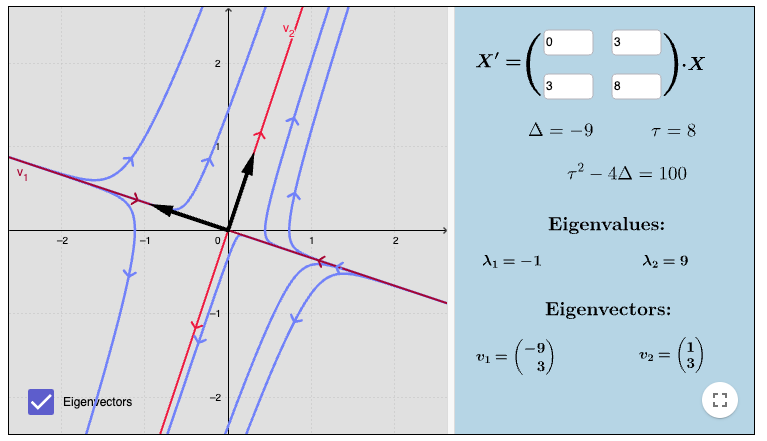
\includegraphics[width=5in]{Images/ImgPhasePlane0338.png}
    %     \end{center}         
    } 
    \else 
        \begin{center}
        \begin{tikzpicture}[scale=0.85]
        \draw[very thick, ->] (-3, 0) -- (3.25, 0);
        \draw[very thick, ->] (0, -3) -- (0, 3.25);
        \end{tikzpicture}
        \end{center}    
        \vspace{2cm}
    \fi        
\end{parts}
% \fi 

% \ifnum \SetNumber=2
%     \question[4] Consider the DE: $y''+4y'+12y=0$. 
\begin{parts}
    \part Solve the DE.

    \ifnum \Solutions=1 {\color{DarkBlue} 
    \textbf{Solutions:} let $y=e^{\lambda t}$.
        \begin{align}
            0 &= \lambda^2 +4\lambda +12 \\
            \lambda &= -2 \pm \frac 12 \sqrt{4^2 - 4 \cdot 12} = -2 \pm \frac 12 \sqrt{-32} = -2 \pm 2\sqrt 2 \\
            y &= c_1 e^{-2t}\cos(2\sqrt2 t) + c_2 \sin(2\sqrt2 t)
        \end{align}
    } 
    \else 
    \vspace{4cm}
    \fi
    
    \part Sketch the phase portrait on the axes below. In you sketch, please: 
    \begin{itemize}
        \item indicate the direction of motion on your solution curves
        \item label your axes
        \item identify the points in the phase portrait the points where $y'' = 0$ 
    \end{itemize} 
    
    \ifnum \Solutions=1 {\color{DarkBlue} 
    \textbf{Solutions:} phase portrait should have axes labeled as $y$ and $y'$, or $x_1$ and $x_2$. Solution curves should be: 
    \begin{itemize}
        \item spirals
        \item moving clockwise
        \item moving towards origin
    \end{itemize}
    To determine where $y''=0$ we can use the DE:
    \begin{align}
        0 &= y''+4y'+12y \\
        0 & = 0 + 4y' +12y \\
        y' &= - 3y
    \end{align}
    Students can either add the line $y'=-3y$ to the graph or write down the equation. 
    
    % Phase diagram below.
        
    %     \begin{center}
    %     % 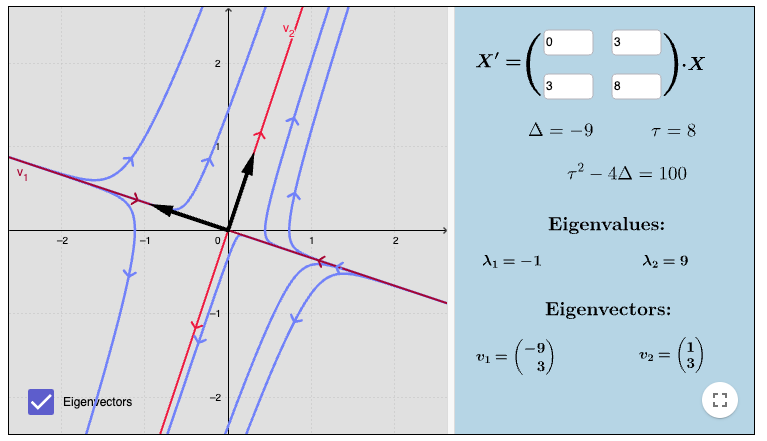
\includegraphics[width=5in]{Images/ImgPhasePlane0338.png}
    %     \end{center}         
    } 
    \else 
        \begin{center}
        \begin{tikzpicture}[scale=0.85]
        \draw[very thick, ->] (-3, 0) -- (3.25, 0);
        \draw[very thick, ->] (0, -3) -- (0, 3.25);
        \end{tikzpicture}
        \end{center}    
        \vspace{2cm}
    \fi        
\end{parts}
%     \question[8] Fill in the blanks. You do not need to show your work. 
%     \begin{parts}
%         \ifnum \Version=1
\part Suppose that we want reflect points in $\mathbb R^2$ across the line $x_1 = 4$. Using homogeneous coordinates we can use a transform of the form $T(\vec x) = A\vec x$, where $\vec x \in \mathbb R^3$ and $A$ is $$A = \begin{pmatrix} 1&0&a_1\\0&1&a_2\\0&0&a_3\end{pmatrix}\begin{pmatrix}b_1&b_2&0\\b_3&b_4&0\\0&0&1 \end{pmatrix}\begin{pmatrix} 1&0&c_1\\0&1&c_2\\0&0&c_3 \end{pmatrix}$$ Then $a_1 = \framebox{\strut\hspace{1.0cm}}$, $a_2 = \framebox{\strut\hspace{1.0cm}}$, $b_1 = \framebox{\strut\hspace{1.0cm}}$, $b_2 = \framebox{\strut\hspace{1.0cm}}$, $c_1 = \framebox{\strut\hspace{1.0cm}}$, $c_2 = \framebox{\strut\hspace{1.0cm}}$.
\ifnum \Solutions=1 {\color{DarkBlue} \textit{Solutions:} 
The matrices we need are
$$A = \begin{pmatrix} 1&0&4\\0&1&0\\0&0&1\end{pmatrix}\begin{pmatrix}-1&0&0\\0&1&0\\0&0&1 \end{pmatrix}\begin{pmatrix} 1&0&-4\\0&1&0\\0&0&1 \end{pmatrix}$$    
So $a_1 = 4, a_2 = 0, b_1 = -1, b_2 = 0, c_1 = -4, c_2 = 0$. 
} 
\fi    
\fi 





\ifnum \Version=2
    \part Suppose $A = \begin{pmatrix} 2&4\\2&5\end{pmatrix}$ and $A^{-1} = \begin{pmatrix} a_1 & a_2 \\ a_3 & a_4 \end{pmatrix}$. Then $a_1 = \framebox{\strut\hspace{1.0cm}}$, $a_2 = \framebox{\strut\hspace{1.0cm}}$, $a_3 = \framebox{\strut\hspace{1.0cm}}$, $a_4 = \framebox{\strut\hspace{1.0cm}}$.
    
    \ifnum \Solutions=1 {\color{DarkBlue} \textit{Solutions:} We can either use the formula for the inverse of a $2\times 2 $ matrix or row reduce the block matrix $\begin{pmatrix} A & I\end{pmatrix}$. The latter yields
    \begin{align}
        \begin{pmatrix} A & I\end{pmatrix} = \begin{pmatrix} 2&4&1&0\\2&5&0&1\end{pmatrix} 
        \sim \begin{pmatrix} 1&2&1/2&0\\0&1&-1&1\end{pmatrix}
        \sim \begin{pmatrix} 1&0&5/2&-2\\0&1&-1&1\end{pmatrix}
    \end{align}
    Thus $A^{-1} =\begin{pmatrix} 5/2&-2\\-1&1\end{pmatrix}$. 
    } 
    \fi        
\fi  

\ifnum \Version=3
    %%% NUMBERS MORE MESSY THAN NECESSARY %%%
    \part Suppose $A$ has the LU factorization $A=LU$, where $L = \begin{pmatrix} 1 & 0 \\ 4 & 1 \end{pmatrix}$ and $U = \begin{pmatrix} 2 & 5 \\ 0 & 4 \end{pmatrix}$. Then the system $Ax=b$ where $b = \begin{pmatrix} 2\\3 \end{pmatrix}$ can be solved using $Ly=b$ and $Ux=y$, with $y = \begin{pmatrix} y_1\\y_2\end{pmatrix}$ and $x= \begin{pmatrix} x_1\\x_2\end{pmatrix}$. Then $y_1 = \framebox{\strut\hspace{1.0cm}}$, $y_2 = \framebox{\strut\hspace{1.0cm}}$, $x_1 = \framebox{\strut\hspace{1.0cm}}$, $x_2 = \framebox{\strut\hspace{1.0cm}}$.

    %%% NUMBERS MORE MESSY THAN NECESSARY %%%    
    \ifnum \Solutions=1 {\color{DarkBlue} \textit{Solutions:} 
    We can solve $Ly=b$ by row reducing the augmented matrix $( L \, | \, b)$.
    $$\begin{pmatrix} 1&0&2\\4&1&3\end{pmatrix} \sim \begin{pmatrix} 1&0&2\\0&1&-5\end{pmatrix}$$
    Thus $y = \begin{pmatrix} 2\\-5\end{pmatrix}$. Solve $Ux=y$ by row reducing the augmented matrix $(U \, | \ y)$. 
    $$\begin{pmatrix} 2&5&2\\0&4&-5\end{pmatrix} 
    \sim \begin{pmatrix} 2&5&2\\0&1&-5/4\end{pmatrix}
    \sim \begin{pmatrix} 2&0&8/4+25/4\\0&1&-5/4\end{pmatrix}
    \sim \begin{pmatrix} 1&0&33/8\\0&1&-5/4\end{pmatrix}
    $$
    Thus $y_1=2, y_2=-5, x_1=33/8, x_2 = -5/4$. 
    } 
    \fi        
\fi  


\ifnum \Version=4
\part If the consumption matrix for an economy is $C=\frac{1}{10}\begin{pmatrix} 2&0\\4&9\end{pmatrix}$ then the output $x$ to meet a desired output $d=\begin{pmatrix} 16\\20\end{pmatrix}$ is $x=\begin{pmatrix} x_1\\x_2 \end{pmatrix}$, where $x_1 = \framebox{\strut\hspace{1.0cm}}$, $x_2 = \framebox{\strut\hspace{1.0cm}}$.

\ifnum \Solutions=1 {\color{DarkBlue} \textit{Solutions:} 
The output we need satisfies 
$$x = d + Cx$$
Which is also
$$(I-C)x = d$$
But 
$$I-C = \begin{pmatrix} 1&0\\0&1\end{pmatrix} - \begin{pmatrix} 0.2 & 0 \\ 0.4 & 0.9 \end{pmatrix} = \begin{pmatrix} 0.8 & 0 \\ -0.4 & 0.1 \end{pmatrix}$$
Thus we can determine $x$ by reducing the augmented matrix below as follows. 
\begin{align}
    \begin{pmatrix} 0.8 & 0 & 16\\ -0.4 &  0.1 & 20\end{pmatrix} 
    & \sim \begin{pmatrix} 8 & 0 & 160\\ -4 & 1 & 200\end{pmatrix} 
     \sim \begin{pmatrix} 1 & 0 & 20\\ -4 & 1 & 200\end{pmatrix} 
     \sim \begin{pmatrix} 1 & 0 & 20\\ 0 & 1 & 280\end{pmatrix} 
\end{align}
Thus $x_1 = 20$, $x_2 = 280$. 
} 
\fi        
\fi        





\ifnum \Version=5
\part Suppose we want to project points in $\mathbb R^2$ onto the line $x_2=4$. Using homogeneous coordinates we can use a transform of the form $T(\vec x) = A\vec x$, where $A$ is $$A = \begin{pmatrix} 1&0&a_1\\0&1&a_2\\0&0&a_3\end{pmatrix}\begin{pmatrix}b_1&b_2&0\\b_3&b_4&0\\0&0&1 \end{pmatrix}\begin{pmatrix} 1&0&c_1\\0&1&c_2\\0&0&c_3 \end{pmatrix}$$
Then $a_1 = \framebox{\strut\hspace{1.0cm}}$, $a_2 = \framebox{\strut\hspace{1.0cm}}$, $b_1 = \framebox{\strut\hspace{1.0cm}}$, $b_2 = \framebox{\strut\hspace{1.0cm}}$, $c_1 = \framebox{\strut\hspace{1.0cm}}$, $c_2 = \framebox{\strut\hspace{1.0cm}}$.
\ifnum \Solutions=1 {\color{DarkBlue} \textit{Solutions:} 
The matrices we need are
$$A = 
\begin{pmatrix} 1&0&0\\0&1&4\\0&0&1\end{pmatrix}
\begin{pmatrix} 1&0&0\\0&0&0\\0&0&1 \end{pmatrix}
\begin{pmatrix} 1&0&0\\0&1&-4\\0&0&1 \end{pmatrix}
$$    
So $a_1 = 0, a_2 = 4, b_1 = 1, b_2 = 0, c_1 = 0, c_2 = -4$. 
} 
\fi        
\fi        
    

        
\ifnum \Version=6
    \part Suppose that we want reflect points in $\mathbb R^2$ across the line $x_2 = 4$. Using homogeneous coordinates we can use a transform of the form $T(\vec x) = A\vec x$, where $\vec x \in \mathbb R^3$ and $A$ is $$A = \begin{pmatrix} 1&0&a_1\\0&1&a_2\\0&0&a_3\end{pmatrix}\begin{pmatrix}b_1&b_2&0\\b_3&b_4&0\\0&0&1 \end{pmatrix}\begin{pmatrix} 1&0&c_1\\0&1&c_2\\0&0&c_3 \end{pmatrix}$$ Then $a_1 = \framebox{\strut\hspace{1.0cm}}$, $a_2 = \framebox{\strut\hspace{1.0cm}}$, $b_1 = \framebox{\strut\hspace{1.0cm}}$, $b_2 = \framebox{\strut\hspace{1.0cm}}$, $c_1 = \framebox{\strut\hspace{1.0cm}}$, $c_2 = \framebox{\strut\hspace{1.0cm}}$.
    
    \ifnum \Solutions=1 {\color{DarkBlue} \textit{Solutions:} 
    The matrices we need are
    $$A = \begin{pmatrix} 1&0&0\\0&1&4\\0&0&1\end{pmatrix}\begin{pmatrix}1&0&0\\0&-1&0\\0&0&1 \end{pmatrix}\begin{pmatrix} 1&0&0\\0&1&-4\\0&0&1 \end{pmatrix}$$    
    } 
    \fi    
\fi 
    
    

\ifnum \Version=7
    \part If the Leontief production equation for an economy with two sectors has consumption matrix $C=\begin{pmatrix}0.4&0\\0.1&0.2 \end{pmatrix}$ and demand vector $\vec d=\begin{pmatrix} 60\\6\end{pmatrix}$ then the production vector has the form $\vec x = \begin{pmatrix} x_1 \\ x_2 \end{pmatrix}$ where $x_1 = \framebox{\strut\hspace{1.25cm}}$ and $x_2 = \framebox{\strut\hspace{1.25cm}}$.
    
    \ifnum \Solutions=1 {\color{DarkBlue} \textit{Solutions:} 
    The production model is $$x = d + Cx$$ Rearranging yields $$(I-C)x = d$$ And $I-C$ is
    \begin{align}
        I -  C = \begin{pmatrix} 1&0\\0&1 \end{pmatrix} - \begin{pmatrix} .4&0\\.1&.2\end{pmatrix} = \begin{pmatrix} .6&0\\-0.1&.8\end{pmatrix} 
    \end{align} 
    Expressing $(I-C)x=d$ as an augmented matrix and reducing gives the solution. 
    \begin{align}
        \begin{pmatrix} .6&0&60\\-0.1&.8&6\end{pmatrix} \sim \begin{pmatrix} 6&0&600\\-1&8&60\end{pmatrix}\sim \begin{pmatrix} 1&0&100\\-1&8&60\end{pmatrix}\sim\begin{pmatrix} 1&0&100\\0&1&20\end{pmatrix}
    \end{align}
    Therefore $x_1=100$, $x_2 = 20$. 
    } 
    \fi        
\fi        



\ifnum \Version=8

    \part If $A$ has LU factorization $A=LU$, where $U = \begin{pmatrix} 2&0\\0&3\end{pmatrix}$, and the solution to $L\vec y = \begin{pmatrix}6\\12 \end{pmatrix}$ is $\vec y = \begin{pmatrix} -2\\27 \end{pmatrix}$, then the solution to $A\vec x = \begin{pmatrix}6\\12 \end{pmatrix}$ is $\vec x = \begin{pmatrix} x_1\\x_2\end{pmatrix}$, where $x_1 = \framebox{\strut\hspace{1.0cm}}$, $x_2 = \framebox{\strut\hspace{1.0cm}}$.
    %
    \ifnum \Solutions=1 {\color{DarkBlue} \textit{Solutions:} 
    If $A\vec x = LU\vec x = \begin{pmatrix} 6\\12 \end{pmatrix}$, and $L\vec y = \begin{pmatrix} 6\\12 \end{pmatrix}$ then $U\vec x = \vec y$. But we are given $\vec y$, so \begin{align} U\vec x = \begin{pmatrix} -2\\27 \end{pmatrix}\end{align} Expressing this as an augmented matrix we obtain 
    $$\begin{pmatrix} 2&0 & -2\\0&3&27 \end{pmatrix}$$
    Thus $x_1 = -1$, $x_2= 27/3 = 9$. 
    } 
    \else
      
    \fi
\fi        




\ifnum \Version=9

\part Suppose we want to use homogeneous coordinates to rotate points in $\mathbb R^2$ counter-clockwise by $\pi/2$ radians about the point $(-1,2)$. We can use a transform of the form $T(\vec x) = A\vec x$, where $A$ is $$A = \begin{pmatrix} 1&0&a_1\\0&1&a_2\\0&0&a_3\end{pmatrix}\begin{pmatrix}b_1&b_2&0\\b_3&b_4&0\\0&0&1 \end{pmatrix}\begin{pmatrix} 1&0&c_1\\0&1&c_2\\0&0&c_3 \end{pmatrix}$$
Then $a_1 = \framebox{\strut\hspace{1.0cm}}$, $a_2 = \framebox{\strut\hspace{1.0cm}}$, $b_1 = \framebox{\strut\hspace{1.0cm}}$, $b_2 = \framebox{\strut\hspace{1.0cm}}$, $c_1 = \framebox{\strut\hspace{1.0cm}}$, $c_2 = \framebox{\strut\hspace{1.0cm}}$.
\ifnum \Solutions=1 {\color{DarkBlue} \textit{Solutions:} 
The matrices we need are
$$A = 
\begin{pmatrix} 1&0&-1\\0&1&2\\0&0&1\end{pmatrix}
\begin{pmatrix} 0&1&0\\-1&0&0\\0&0&1 \end{pmatrix}
\begin{pmatrix} 1&0&1\\0&1&-2\\0&0&1 \end{pmatrix}
$$    
So $a_1 = 1, a_2 = 0, b_1 = 0, b_2 = 1, c_1 = 1, c_2 = 0$. 
} 
\fi        
\fi        



\ifnum \Version=10

\part Suppose we want to use homogeneous coordinates to rotate points in $\mathbb R^2$ clockwise by $\pi/2$ radians about the point $(2,1)$. We can use a transform of the form $T(\vec x) = A\vec x$, where $A$ is $$A = \begin{pmatrix} 1&0&a_1\\0&1&a_2\\0&0&a_3\end{pmatrix}\begin{pmatrix}b_1&b_2&0\\b_3&b_4&0\\0&0&1 \end{pmatrix}\begin{pmatrix} 1&0&c_1\\0&1&c_2\\0&0&c_3 \end{pmatrix}$$
Then $a_1 = \framebox{\strut\hspace{1.0cm}}$, $a_2 = \framebox{\strut\hspace{1.0cm}}$, $b_1 = \framebox{\strut\hspace{1.0cm}}$, $b_2 = \framebox{\strut\hspace{1.0cm}}$, $c_1 = \framebox{\strut\hspace{1.0cm}}$, $c_2 = \framebox{\strut\hspace{1.0cm}}$.
\ifnum \Solutions=1 {\color{DarkBlue} \textit{Solutions:} 
The matrices we need are
$$A = 
\begin{pmatrix} 1&0&2\\0&1&1\\0&0&1\end{pmatrix}
\begin{pmatrix} 0&1&0\\-1&0&0\\0&0&1 \end{pmatrix}
\begin{pmatrix} 1&0&-2\\0&1&-1\\0&0&1 \end{pmatrix}
$$    
So $a_1 = 2, a_2 = 1, b_1 = 0, b_2 = 1, c_1 = -2, c_2 = -1$. 
} 
\fi    
\fi   



\ifnum \Version=11
\part If the LU factorization is $A=LU$, where $U$ is obtained by applying one row operation to $A$, and $A = \begin{pmatrix} 1&2&1\\8&20&50\end{pmatrix}$. Then $L = \begin{pmatrix} 1& 0\\l_1 & 1 \end{pmatrix} $ and $U= \begin{pmatrix} 1&2 & 4\\u_1 & u_2 & u_3 \end{pmatrix}$, where $l_1 = \framebox{\strut\hspace{1.25cm}}$, $u_1 = \framebox{\strut\hspace{1.25cm}}$, $u_2 = \framebox{\strut\hspace{1.25cm}}$ and $u_3 = \framebox{\strut\hspace{1.25cm}}$.
\ifnum \Solutions=1 {\color{DarkBlue} \textit{Solutions:} 
To reduce $A$ to $U$ we need exactly one row operation, $R_2 - 8R_1 \to R_2$. That row operation applied to $A$ gives us NEED TO FIX THIS PART $$ U = \begin{pmatrix} 2&3\\0&3\end{pmatrix}$$. So $u_1 = 2, u_2 = 3, u_3=0, u_4 = 3$. 
} 
\fi        
\fi        


\ifnum \Version=12

\part If $A$ has LU factorization $A=LU$, where $U = \begin{pmatrix} 2&1\\0&3\end{pmatrix}$, and the solution to $L\vec y = \begin{pmatrix}6\\12 \end{pmatrix}$ is $\vec y = \begin{pmatrix} 2\\24 \end{pmatrix}$, then the solution to $A\vec x = \begin{pmatrix}6\\12 \end{pmatrix}$ is $\vec x = \begin{pmatrix} x_1\\x_2\end{pmatrix}$, where $x_1 = \framebox{\strut\hspace{1.0cm}}$, $x_2 = \framebox{\strut\hspace{1.0cm}}$.
\ifnum \Solutions=1 {\color{DarkBlue} \textit{Solutions:} 
If $A\vec x = LU\vec x = \begin{pmatrix} 6\\12 \end{pmatrix}$, and $L\vec y = \begin{pmatrix} 6\\12 \end{pmatrix}$ then $U\vec x = \vec y$. But we are given $\vec y$, so \begin{align} U\vec x = \begin{pmatrix} 2\\24 \end{pmatrix}\end{align} Expressing this as an augmented matrix we obtain 
$$\begin{pmatrix} 2&0 & 2\\0&3&24 \end{pmatrix}$$
Thus $x_1 = 1$, $x_2= 24/3 = 8$. 
} 
\else
  
\fi
\fi       

\ifnum \Version=13
\part If $A$ has LU factorization $A=LU$, where $U = \begin{pmatrix} 2&0\\0&3\end{pmatrix}$, and the solution to $L\vec y = \begin{pmatrix}6\\12 \end{pmatrix}$ is $\vec y = \begin{pmatrix} 2\\24 \end{pmatrix}$, then the solution to $A\vec x = \begin{pmatrix}6\\12 \end{pmatrix}$ is $\vec x = \begin{pmatrix} x_1\\x_2\end{pmatrix}$, where $x_1 = \framebox{\strut\hspace{1.0cm}}$, $x_2 = \framebox{\strut\hspace{1.0cm}}$.
\ifnum \Solutions=1 {\color{DarkBlue} \textit{Solutions:} 
If $A\vec x = LU\vec x = \begin{pmatrix} 6\\12 \end{pmatrix}$, and $L\vec y = \begin{pmatrix} 6\\12 \end{pmatrix}$ then $U\vec x = \vec y$. But we are given $\vec y$, so \begin{align} U\vec x = \begin{pmatrix} 2\\24 \end{pmatrix}\end{align} Expressing this as an augmented matrix we obtain 
$$\begin{pmatrix} 2&0 & 2\\0&3&24 \end{pmatrix}$$
Thus $x_1 = 1$, $x_2= 24/3 = 8$. 
} 
\else
\fi
\fi    


\ifnum \Version=14
\part If $A = \begin{pmatrix} 2&3\\4&9 \end{pmatrix}$ has the LU factorization $A=LU$, where $L = \begin{pmatrix} 1 & 0 \\ l_1 & 1 \end{pmatrix}$ and $U = \begin{pmatrix} u_1 & u_2 \\ u_3 & u_4 \end{pmatrix}$, then $l_1 = \framebox{\strut\hspace{1.0cm}}$, $u_1 = \framebox{\strut\hspace{1.0cm}}$, $u_2 = \framebox{\strut\hspace{1.0cm}}$, $u_3 = \framebox{\strut\hspace{1.0cm}}$,$u_4 = \framebox{\strut\hspace{1.0cm}}$.
\ifnum \Solutions=1 {\color{DarkBlue} \textit{Solutions:} 
To reduce $A$ to $U$ we need exactly one row operation, $R_2 - 2R_1 \to R_2$. That row operation applied to $A$ gives us $$ U = \begin{pmatrix} 2&3\\0&3\end{pmatrix}$$. So $u_1 = 2, u_2 = 3, u_3=0, u_4 = 3$. 
} 
\fi        
\fi   % 2
%         \ifnum \Version=1

    \part $A\!= \! \begin{pmatrix} 2&6\\2&6\end{pmatrix}$ is row equivalent to $E\!=\!\begin{pmatrix} 1&3\\0&0\end{pmatrix}$. A basis for $\Col A$ is $\vec x = \begin{pmatrix} 1\\k \end{pmatrix}$, where $k = \framebox{\strut\hspace{0.8cm}}$. 
    
    \ifnum \Solutions=1 {\color{DarkBlue} \textit{Solutions.} 
    We are given the vector $\begin{pmatrix} 1\\k\end{pmatrix}$ which is a basis for $\Col A$ for $k=1$, because every column is in the span of $\begin{pmatrix} 1\\1\end{pmatrix}$.
    } 
   \fi

\fi


\ifnum \Version=2

    \part Suppose $A$, $B$, and $C$ are $2\times2$ matrices, $A = BC$, and $\Null B$ is the line $x_1=0$. If $T(\vec x)=C\vec x$ rotates vectors clockwise by $\pi/2$ radians about the origin, then $\Null A$ is spanned by $\vec y = \begin{pmatrix} y_1\\y_2\end{pmatrix}$ where $y_1 = \framebox{\strut\hspace{1.0cm}}$ and $y_2 = \framebox{\strut\hspace{1.0cm}}$. Please use numbers for $y_1$ and $y_2$ (not variables). 
    
    \ifnum \Solutions=1 {\color{DarkBlue} \textit{Solutions.} 
    Note that the line $x_1=0$ is the $x_2$-axis, and that there are a few ways to approach this problem. Here are two different methods. 
    \begin{itemize}
        \item \textbf{Method 1}: The transform $T(x) = Ax = BCx$ first rotates vectors clockwise by $\pi/2$ radians about the origin. Any vector on the $x_1$-axis gets rotated to the $x_2$-axis. Vectors on the $x_1$-axis are in the span of $y = \begin{pmatrix} 1\\0 \end{pmatrix}$. So any vector in the span of $y$ is rotated into $\Null B$, so $BCy = 0$. But $A=BC$ so $\Null A$ is spanned by $y = \begin{pmatrix} 1\\0\end{pmatrix}$. We can choose $y_1 = 1$ and $y_2=0$. 
        \item \textbf{Method 2}: The transform $T(x) = Ax = BCx$ first rotates vectors clockwise by $\pi/2$ radians about the origin. In other words, $C$ will transform $e_1 = \begin{pmatrix} 1\\0 \end{pmatrix}$ to $T_C(e_1) = \begin{pmatrix} 0\\-1 \end{pmatrix}$, and $e_2 = \begin{pmatrix} 0\\ 1 \end{pmatrix}$ to $T_C(e_2) = \begin{pmatrix} 1\\0 \end{pmatrix}$. This means that the standard matrix of the transform $T_C$ is $C = \begin{pmatrix} 0&1\\-1&0\end{pmatrix}$, and $C$ will transform a vector of the form $\begin{pmatrix}x_1\\x_2 \end{pmatrix}$ to $\begin{pmatrix} x_2 \\ -x_1\end{pmatrix}$. But $\Null B$ is the line spanned by $\begin{pmatrix} 0\\1\end{pmatrix}$, so $T_C(x)$ is in $\Null B$ when $x_2 = 0$. So $y = \begin{pmatrix} x_1 \\ x_2 \end{pmatrix} = \begin{pmatrix}x_1\\0 \end{pmatrix}$. So we can choose $y_1 = 1$ and $y_2 = 0$. 
    \end{itemize}
    Do not leave your answer as $y_1 = x_1$ and $y_2=0$ because then you haven't specified that $x_1 \ne 0$. 
    } 
    
    \fi    
\fi




\ifnum \Version=3

    \part A basis for the subspace $S = \{ \vec x \in \mathbb R^2 \, | \, x_1=3x_2 \}$ is $\vec x = \begin{pmatrix} k\\1 \end{pmatrix}$, where $k = \framebox{\strut\hspace{0.8cm}}$. 
    
    \ifnum \Solutions=1 {\color{DarkBlue} \textit{Solutions.} 
    We are given the vector $\begin{pmatrix} k\\1 \end{pmatrix}$ which is in $S$ for $k=3$, and $\Dim S = 1$ so $\begin{pmatrix} 3\\1 \end{pmatrix}$ is a basis for $S$.
    } 
   \fi

\fi


\ifnum \Version=4

    \part Suppose $A$, $B$, and $C$ are $2\times2$ matrices, $A = BC$, and $\Null B$ is the line $x_2=0$. If $T(\vec x)=C\vec x$ reflects vectors through the line $x_1+x_2= 0$, then $\Null A$ is spanned by the vector $\vec y = \begin{pmatrix} y_1\\y_2\end{pmatrix}$ where $y_1 = \framebox{\strut\hspace{1.0cm}}$ and $y_2 = \framebox{\strut\hspace{1.0cm}}$. 
    
    \ifnum \Solutions=1 {\color{DarkBlue} \textit{Solutions.} 
    
    We seek the vectors that are mapped by $T$ onto the null space of $B$. We know that $T$ is a reflection through the line $x_2=-x_1$, so $T$ maps vectors of the form $v = \begin{pmatrix} 0\\ k \end{pmatrix}$ onto the $x_1$-axis (which is the line $x_2=0$). In other words, 
    $$Cv = C \begin{pmatrix} 0\\k\end{pmatrix}$$
    will be a point on the $x_1$-axis. Then
    $$Av = BCv=B(Cv)$$
    will be a zero vector, because $Cv$ is in the null space of $B$. So a basis for the null space of $A$ is $v = \begin{pmatrix} 0 \\ 1 \end{pmatrix}$. Because any vector in the span of $v$ satisfies $Av = BCv = 0$. 
    
    Note that there are other valid approaches to this problem. We could also construct both matrices $B$ and $C$, compute their product which is $A$, and then determine a basis for the null space of $A$. 
    } 
    
    \fi    
\fi

\ifnum \Version=5

    \part A basis for the subspace $S = \{ \vec x \in \mathbb R^2 \, | \, x_1=3x_2 \}$ is $\vec x = \begin{pmatrix} k\\1 \end{pmatrix}$, where $k = \framebox{\strut\hspace{0.8cm}}$. 
    
    \ifnum \Solutions=1 {\color{DarkBlue} \textit{Solutions.} 
    We are given the vector $\begin{pmatrix} k\\1 \end{pmatrix}$ which is in $S$ for $k=3$, and $\Dim S = 1$ so $\begin{pmatrix} 3\\1 \end{pmatrix}$ is a basis for $S$. The only correct answer to this question is $k=3$. 
    } 
   \fi

\fi


\ifnum \Version=6

    \part $A\!= \! \begin{pmatrix} 2&6\\2&6\end{pmatrix}$ is row equivalent to $E\!=\!\begin{pmatrix} 1&3\\0&0\end{pmatrix}$. A basis for $\Col A$ is $\vec x = \begin{pmatrix} 1\\k \end{pmatrix}$, where $k = \framebox{\strut\hspace{0.8cm}}$. 
    
    \ifnum \Solutions=1 {\color{DarkBlue} \textit{Solutions.} 
    We are given the vector $\begin{pmatrix} 1\\k\end{pmatrix}$ which is a basis for $\Col A$ for $k=1$, because every column is in the span of $\begin{pmatrix} 1\\1\end{pmatrix}$.
    } 
   \fi

\fi      


\ifnum \Version=7

    \part Suppose $A$, $B$, and $C$ are $2\times2$ matrices, $A = BC$, and $\Null B$ is the line $x_1=0$. If $T(\vec x)=C\vec x$ reflects vectors through the line $x_1+x_2= 0$, then $\Null A$ is spanned by the vector $\vec y = \begin{pmatrix} y_1\\y_2\end{pmatrix}$ where $y_1 = \framebox{\strut\hspace{1.0cm}}$ and $y_2 = \framebox{\strut\hspace{1.0cm}}$. Please use numbers for $y_1$ and $y_2$ (not variables). 
    
    \ifnum \Solutions=1 {\color{DarkBlue} \textit{Solutions.} 
    Any vector in the span of $v = \begin{pmatrix} k\\0\end{pmatrix}$, where $k \ne 0$ will be reflected by $C$ onto the $x_2$ axis where $x_1 = 0$. That is, if $y$ is in the span of $v$, then $BCy = 0$. So $y_1$ can be any non-zero number, and $y_2 = 0$. We can choose $y_1 = 1$. 
    } 
    
    \fi    
\fi


\ifnum \Version=8

    \part $A\!= \! \begin{pmatrix} 1&4\\2&8\end{pmatrix}$ is row equivalent to $E\!=\!\begin{pmatrix} 1&2\\0&0\end{pmatrix}$. A basis for $\Col A$ is $\vec x = \begin{pmatrix} 1\\k \end{pmatrix}$, where $k = \framebox{\strut\hspace{0.8cm}}$. 
    
    \ifnum \Solutions=1 {\color{DarkBlue} \textit{Solutions.} 
    The columns of $A$ are spanned by $\begin{pmatrix} 1\\2\end{pmatrix}$, 
    so $k=2$. 
    } 
   \fi

\fi      





\ifnum \Version=9

    \part A basis for the subspace $S = \{ \vec x \in \mathbb R^2 \, | \, x_1=2x_2 \}$ is $\vec x = \begin{pmatrix} k & 1 \end{pmatrix}^T$, where $k = \framebox{\strut\hspace{0.8cm}}$. 
    
    \ifnum \Solutions=1 {\color{DarkBlue} \textit{Solutions.} 
    We are given the vector $\begin{pmatrix} k\\1 \end{pmatrix}$ which is in $S$ for $k=2$, and $\Dim S = 1$ so $\begin{pmatrix} 2\\1 \end{pmatrix}$ is a basis for $S$.
    } 
   \fi

\fi % 2
%         \ifnum \Version=1
    \part Matrix $A$ is $2\times2$, $\Col A$ is the line $x_1=2x_2$, $\Null A$ is the line $x_1=-x_2$, then $A=\begin{pmatrix} a_1 & a_2 \\ a_3 & a_4 \end{pmatrix} $ where 
        $a_1 = \framebox{\strut\hspace{1.0cm}}$, 
        $a_2 = \framebox{\strut\hspace{1.0cm}}$, 
        $a_3 = \framebox{\strut\hspace{1.0cm}}$, 
        $a_4 = \framebox{\strut\hspace{1.0cm}}$.
        
    \ifnum \Solutions=1 {\color{DarkBlue} \textit{Solutions:} 
    If $\Col A$ is the line $x_1=2x_2$ then a vector in $\Col A$ is $\begin{pmatrix} 2\\1\end{pmatrix}$ because if $x_2=1$, then $x_1=2$. Then the first column of $A$ can be $\begin{pmatrix} 2\\1\end{pmatrix}$ or $A = \begin{pmatrix} 2&c_1\\1&c_2\end{pmatrix}$. We need to work out what $c_1$ and $c_2$ are, but if $\Null A$ is the line $x_1+x_2=0$ then a vector in the null space of $A$ is $v = \begin{pmatrix} -1\\1\end{pmatrix}$, so $$Av = \begin{pmatrix}2&c_1\\1&c_2 \end{pmatrix}\begin{pmatrix} -1\\1\end{pmatrix} = \begin{pmatrix} 0\\0\end{pmatrix}$$ This gives us $c_1 = 2$, $c_2 = 1$, so $A = \begin{pmatrix} 2&2\\1&1\end{pmatrix}$, but any non-zero scalar multiple of this matrix also works. 
    } 
   \else
   \fi                
\fi
    



\ifnum \Version=2
    \part Matrix $A$ is $2\times2$, $\Col A$ is spanned by $\begin{pmatrix} 1\\2\end{pmatrix}$, $\Null A$ is the line $x_1=-x_2$, then $A=\begin{pmatrix} a_1 & a_2 \\ a_3 & a_4 \end{pmatrix} $ where 
        $a_1 = \framebox{\strut\hspace{1.0cm}}$, 
        $a_2 = \framebox{\strut\hspace{1.0cm}}$, 
        $a_3 = \framebox{\strut\hspace{1.0cm}}$, 
        $a_4 = \framebox{\strut\hspace{1.0cm}}$.
    \ifnum \Solutions=1 {\color{DarkBlue} \textit{Solutions:} 
    A vector in $\Col A$ is $\begin{pmatrix} 1\\2\end{pmatrix}$. Then the first column of $A$ can be $\begin{pmatrix} 1\\2\end{pmatrix}$ or $A = \begin{pmatrix} 1&c_1\\2&c_2\end{pmatrix}$. We need to work out what $c_1$ and $c_2$ are, but if $\Null A$ is the line $x_1+x_2=0$ then a vector in the null space of $A$ is $v = \begin{pmatrix} -1\\1\end{pmatrix}$, so $$Av = \begin{pmatrix}1&c_1\\2&c_2 \end{pmatrix}\begin{pmatrix} -1\\1\end{pmatrix} = \begin{pmatrix} 0\\0\end{pmatrix}$$ This gives us $c_1 = 1$, $c_2 = 2$, so $A = \begin{pmatrix} 1&1\\2&2\end{pmatrix}$, but any non-zero scalar multiple of this matrix also works. For example we could have also used any of the matrices below. 
    $$\begin{pmatrix} 1&1\\2&2\end{pmatrix} , \begin{pmatrix} 2&2\\4&4\end{pmatrix},\begin{pmatrix} 10&10\\20&20\end{pmatrix} , \ldots $$
    } 
   \else
   \fi                  
\fi
    
    
    
    
\ifnum \Version=3
    \part If matrix $A$ is $2\times2$, $\Col A$ is the line $x_2 =0$ and $\Null A$ is the line $x_1=-2x_2$, then $A=\begin{pmatrix} a_1 & a_2 \\ a_3 & a_4 \end{pmatrix} $ where 
        $a_1 = \framebox{\strut\hspace{1.0cm}}$, 
        $a_2 = \framebox{\strut\hspace{1.0cm}}$, 
        $a_3 = \framebox{\strut\hspace{1.0cm}}$, 
        $a_4 = \framebox{\strut\hspace{1.0cm}}$.
        
    \ifnum \Solutions=1 {\color{DarkBlue} \textit{Solutions:} 
    If the column space is the $x_1$-axis then matrix has the form $$A= \begin{pmatrix} a&b\\0&0\end{pmatrix}$$ 
    where $a$ and $b$ are real numbers. If $\Nul A$ is the line $x_1=-2x_2$ then $\begin{pmatrix}-2\\1 \end{pmatrix}$ is in the null space and $$\begin{pmatrix} a&b\\0&0 \end{pmatrix}\begin{pmatrix}-2\\1 \end{pmatrix} = \begin{pmatrix} 0\\0\end{pmatrix}$$ So $-2a+b=0$, and we can choose $a=1$ and $b=2$. So we can set $$a_1=1, a_2 = 2, a_3 =0, a_4=0$$ There are other choices for $a_1, a_2$ that we can use but we must have that $a_3=a_4=0$. 
    } 
   \else
   \fi           
\fi   


\ifnum \Version=4
    \part If matrix $A$ is $2\times2$, $\Col A$ is the line $x_2 =0$ and $\Null A$ is the line $x_1=-2x_2$, then $A=\begin{pmatrix} a_1 & a_2 \\ a_3 & a_4 \end{pmatrix} $ where 
        $a_1 = \framebox{\strut\hspace{1.0cm}}$, 
        $a_2 = \framebox{\strut\hspace{1.0cm}}$, 
        $a_3 = \framebox{\strut\hspace{1.0cm}}$, 
        $a_4 = \framebox{\strut\hspace{1.0cm}}$.
        
    \ifnum \Solutions=1 {\color{DarkBlue} \textit{Solutions:} 
    If the column space is the $x_1$-axis then matrix has the form $$A= \begin{pmatrix} a&b\\0&0\end{pmatrix}$$ 
    where $a$ and $b$ are real numbers. If $\Nul A$ is the line $x_1=-2x_2$ then $\begin{pmatrix}-2\\1 \end{pmatrix}$ is in the null space and $$\begin{pmatrix} a&b\\0&0 \end{pmatrix}\begin{pmatrix}-2\\1 \end{pmatrix} = \begin{pmatrix} 0\\0\end{pmatrix}$$ So $-2a+b=0$, and we can choose $a=1$ and $b=2$. So we can set $$a_1=1, a_2 = 2, a_3 =0, a_4=0$$ There are other choices for $a_1, a_2$ that we can use but we must have that $a_3=a_4=0$. 
    } 
   \else
   \fi           
\fi   



\ifnum \Version=5
    \part Matrix $A$ is $2\times2$, $\Col A$ is the line $x_1=8x_2$, $\Null A$ is the line $x_1+4x_2=0$, then $A=\begin{pmatrix} a_1 & a_2 \\ 1 & a_4 \end{pmatrix} $ where 
    $a_1 = \framebox{\strut\hspace{1.0cm}}$, 
    $a_2 = \framebox{\strut\hspace{1.0cm}}$, 
    $a_4 = \framebox{\strut\hspace{1.0cm}}$.
        
    \ifnum \Solutions=1 {\color{DarkBlue} \textit{Solutions:} 
    If $\Col A$ is the line $x_1=8x_2$ then a vector in $\Col A$ is $\begin{pmatrix} 8\\1\end{pmatrix}$ because if $x_2=1$, then $x_1=8$. Then the first column of $A$ can be $\begin{pmatrix} 8\\1\end{pmatrix}$ or $A = \begin{pmatrix} 8&c_1\\1&c_2\end{pmatrix}$. We need to work out what $c_1$ and $c_2$ are, but if $\Null A$ is the line $x_1+4x_2=0$ then a vector in the null space of $A$ is $v = \begin{pmatrix} 4\\-1\end{pmatrix}$. Because if $x_2=-1$, $x_1=4$. So $$Av = \begin{pmatrix}8&c_1\\1&c_2 \end{pmatrix}\begin{pmatrix} 4\\-1\end{pmatrix} = \begin{pmatrix} 0\\0\end{pmatrix}$$ This gives us $c_1 = 32$, $c_2 = 4$, so 
    $$A = \begin{pmatrix} 8&32\\1&4\end{pmatrix}$$ We are forced to have the entry in the lower left be 1, so this is the only possible answer. 

    } 
   \else
      
   \fi        
\fi   



\ifnum \Version=6
    \part If matrix $A$ is $2\times2$, upper triangular, and $\Null A$ is the line $x_1=-x_2$, then $A=\begin{pmatrix} a_1 & 1 \\ a_3 & a_4 \end{pmatrix} $ where 
        $a_1 = \framebox{\strut\hspace{1.0cm}}$, 
        $a_3 = \framebox{\strut\hspace{1.0cm}}$, 
        $a_4 = \framebox{\strut\hspace{1.0cm}}$.
        
    \ifnum \Solutions=1 {\color{DarkBlue} \textit{Solutions:} 
    If $\Null A$ is the line $x_1=-x_2$ then a vector in $\Nul A$ is $\begin{pmatrix} 1\\-1\end{pmatrix}$. Then the first row of $A$ can be $\begin{pmatrix} 1&1 \end{pmatrix}$ so $A = \begin{pmatrix}1&1\\c_1&c_2\end{pmatrix}$. We need to work out what $c_1$ and $c_2$ are, but if $\Null A$ is a line and $A$ is upper triangular, then $c_1=c_2=0$. This gives us
    $A = \begin{pmatrix} 1&1\\0&0\end{pmatrix}$. This is the only possible answer. So $a_1=1$, $a_3=a_4=0$. 

    } 
   \else
      
   \fi            
\fi   


\ifnum \Version=7
    \part If matrix $A$ is $2\times2$, $\Col A$ is the $x_1$-axis, and $\Null A$ is the line $x_1=-2x_2$, then $A=\begin{pmatrix} 1 & a_2 \\ a_3 & a_4 \end{pmatrix} $ where 
        $a_2 = \framebox{\strut\hspace{1.0cm}}$, 
        $a_3 = \framebox{\strut\hspace{1.0cm}}$, 
        $a_4 = \framebox{\strut\hspace{1.0cm}}$.
        
    \ifnum \Solutions=1 {\color{DarkBlue} \textit{Solutions:} 
    If the column space is the $x_1$-axis then matrix has the form $$A= \begin{pmatrix} a&b\\0&0\end{pmatrix}$$ 
    where $a$ and $b$ are real numbers. We are told that $a=1$, and need to determine $b$. If $\Nul A$ is the line $x_1=-2x_2$ then $\begin{pmatrix}-2\\1 \end{pmatrix}$ is in the null space and $$\begin{pmatrix} 1&b\\0&0 \end{pmatrix}\begin{pmatrix}-2\\1 \end{pmatrix} = \begin{pmatrix} 0\\0\end{pmatrix}$$ So $-2+b=0$, or $b=2$. So we must set $$a_1=1, a_2 = 2, a_3 =0, a_4=0$$ There no are other choices for $a_1, a_2$ and we must have that $a_3=a_4=0$. 
    } 
   \else
   \fi           
\fi   


\ifnum \Version=8
    \part If matrix $A$ is $2\times2$, $\Col A$ is the line $x_2 =0$ and $\Null A$ is the line $x_1=-4x_2$, then $A=\begin{pmatrix} 1 & a_2 \\ a_3 & a_4 \end{pmatrix} $ where 
        $a_1 = \framebox{\strut\hspace{1.0cm}}$, 
        $a_2 = \framebox{\strut\hspace{1.0cm}}$, 
        $a_3 = \framebox{\strut\hspace{1.0cm}}$, 
        $a_4 = \framebox{\strut\hspace{1.0cm}}$.
        
    \ifnum \Solutions=1 {\color{DarkBlue} \textit{Solutions:} 
    If the column space is the $x_1$-axis then matrix has the form $$A= \begin{pmatrix} a&b\\0&0\end{pmatrix}$$ 
    where $a$ and $b$ are real numbers. If $\Nul A$ is the line $x_1=-4x_2$ then $\begin{pmatrix}-4\\1 \end{pmatrix}$ is in the null space and $$\begin{pmatrix} a&b\\0&0 \end{pmatrix}\begin{pmatrix}-4\\1 \end{pmatrix} = \begin{pmatrix} 0\\0\end{pmatrix}$$ So $-4a+b=0$, and we can choose $a=1$ and $b=4$. So we can set $$a_1=1, \ a_2 = 4,\  a_3 =0, \ \textbf{}a_4=0$$ We are told that $a_1 = 1$ so this is the only possible answer. 
    } 
   \else
   \fi           
\fi   
 % 2
%         \ifnum \Version=1
    \part The dimension of the subspace $\{\vec x \in \mathbb R^4 \, | \, x_1-x_3 = 0\}$ is $\framebox{\strut\hspace{1.0cm}}$. 
    
    \ifnum \Solutions=1 {\color{DarkBlue} \textit{Solutions:} The dimension is $3$. 
    } 
   \fi
\fi
    
\ifnum \Version=2
    \part The dimension of the column space of $A=\begin{pmatrix} 1&0&1\\0&1&1\\1&1&2\end{pmatrix}$ is $\framebox{\strut\hspace{1.0cm}}$. 
    
    \ifnum \Solutions=1 {\color{DarkBlue} \textit{Solutions.} 

    By inspection the third column is the sum of the first two, and the first two columns are independent. So $A$ has two pivots, and the number of pivots is the rank, so $\Rank A = 2$. Alternatively we could also row reduce the matrix and find that there are only two pivots, and so the rank must be two. 
    } 
   \else
      
   \fi    
\fi
    
\ifnum \Version=3
    \part The dimension of the subspace $\{\vec x \in \mathbb R^6 \, | \, x_1-x_3 = 0, \, x_2-x_4=0\}$ is $\framebox{\strut\hspace{1.0cm}}$.    
    
    \ifnum \Solutions=1 {\color{DarkBlue} \textit{Solutions:} The dimension is $4$. Note we are told that 
    $$x_1 - x_3 = 0, \ x_2-x_4 =0$$
    But these conditions can be written as
    $$x_1 = x_3 , \ x_2 = x_4 $$
    So vectors in the space have the form 
    $$ x 
    = \begin{pmatrix} x_1 \\ x_2 \\ x_3 \\ x_4 \\ x_5 \\ x_6 \end{pmatrix} 
    = \begin{pmatrix} x_3 \\ x_4 \\ x_3 \\ x_4 \\ x_5 \\ x_6 \end{pmatrix}
    = x_3\begin{pmatrix} 1 \\ 0 \\ 1 \\ 0\\ 0 \\ 0 \end{pmatrix} 
    + x_4\begin{pmatrix}  0 \\ 1 \\ 0\\ 1 \\ 0 \\ 0 \end{pmatrix}
    + x_5\begin{pmatrix}  0 \\ 0 \\ 0\\ 0 \\ 1 \\ 0 \end{pmatrix}
    + x_6\begin{pmatrix}  0 \\ 0 \\ 0\\ 0 \\ 0 \\ 1 \end{pmatrix}
    $$
    From our parametric vector form we see that the following set of vectors are in the subspace and are independent. 
    $$
    \left\{
    \begin{pmatrix} 1 \\ 0 \\ 1 \\ 0\\ 0 \\ 0 \end{pmatrix},
    \begin{pmatrix}  0 \\ 1 \\ 0\\ 1 \\ 0 \\ 0 \end{pmatrix},
    \begin{pmatrix}  0 \\ 0 \\ 0\\ 0 \\ 1 \\ 0 \end{pmatrix},
    \begin{pmatrix}  0 \\ 0 \\ 0\\ 0 \\ 0 \\ 1 \end{pmatrix}
    \right\}
    $$
    Note that each vector satisfies the given conditions because 
    \begin{itemize}
        \item each vector is in $\mathbb R^6$
        \item each vector satisfies $x_1 - x_3 = 0$
        \item each vector satisfies $x_2-x_4 =0$
    \end{itemize}
    There are four vectors in this set, they are independent, and they span the set. The dimension of a space is the number of vectors needed to form a basis for it, so the dimension is 4. 
    } 
   \fi
\fi
    
\ifnum \Version=4
\part How many vectors are needed to form a basis for the subspace $\{\vec x \in \mathbb R^4 \, | \, x_1+x_2 = 0\}$? $\framebox{\strut\hspace{1.0cm}}$. 

    \ifnum \Solutions=1 {\color{DarkBlue} \textit{Solutions.} 
    $3$. 
    } 
   \else
   \fi
\fi
    
\ifnum \Version=5
    \part The dimension of the column space of $A=\begin{pmatrix} 1&0&1\\0&1&1\\1&1&2\end{pmatrix}$ is $\framebox{\strut\hspace{1.0cm}}$. 
    
    \ifnum \Solutions=1 {\color{DarkBlue} \textit{Solutions.} 

    By inspection the third column is the sum of the first two, and the first two columns are independent. So $A$ has two pivots, and the number of pivots is the rank, so $\Rank A = 2$. 
    } 
   \else
      
   \fi    
\fi
    
\ifnum \Version=6
    \part How many vectors are needed to form a basis for the subspace $\{\vec x \in \mathbb R^5 \, | \, x_1+x_2 = 0\}$? $\framebox{\strut\hspace{1.0cm}}$. 
    \ifnum \Solutions=1 {\color{DarkBlue} \textit{Solutions.} 
    $4$. Vectors in the subspace have the general form 
    $$x 
    = \begin{pmatrix} x_1\\x_2\\x_3\\x_4\\x_5\end{pmatrix} 
    = \begin{pmatrix} -x_2\\x_2\\x_3\\x_4\\x_5\end{pmatrix}
    =x_2\begin{pmatrix} -1\\1\\0\\0\\0\end{pmatrix}
    +x_3\begin{pmatrix} 0\\0\\1\\0\\0\end{pmatrix}
    +x_4\begin{pmatrix} 0\\0\\0\\1\\0\end{pmatrix}
    +x_5\begin{pmatrix} 0\\0\\0\\0\\1\end{pmatrix}
    $$
    There are 4 independent vectors in the basis for this subspace. 
    } 
   \else
   \fi    
\fi


\ifnum \Version=7
\part Suppose $S$ is the subspace $S=\{\vec x \in \mathbb R^5 \, | \, x_1+x_2 = 0, x_3+x_4 = 0\}$. How many vectors are needed to form a basis for $S$? $\framebox{\strut\hspace{1.0cm}}$. 

    \ifnum \Solutions=1 {\color{DarkBlue} \textit{Solutions.} 
    $S$ is determined by two linear conditions and vectors in $S$ live in $\mathbb R^5$.  Hence, $S$ is three dimensional.  $x_1$ is free, but not $x_2$. $x_3$ is free, but not $x_4$, and then $x_5$ is free.  A general vector in $S$ is 
    \begin{equation}
        \begin{pmatrix}
            x_1 \\ - x_1 \\ x_3 \\ - x_3 \\ x_5 
        \end{pmatrix} = x_1 \begin{pmatrix}1\\-1\\0\\0\\0 \end{pmatrix}+x_3\begin{pmatrix}0\\0\\1\\-1\\0 \end{pmatrix}+ x_5\begin{pmatrix} 0 \\0\\0\\0\\1 \end{pmatrix}
    \end{equation}
    There are 3 independent vectors in the basis for this subspace.     
    } 
   \else
   \fi
\fi        

\ifnum \Version=8
\part Suppose $S$ is the subspace $S=\{\vec x \in \mathbb R^6 \, | \, x_1+x_2 = 0, x_3+2x_4 = 0\}$. How many vectors are needed to form a basis for $S$? $\framebox{\strut\hspace{1.0cm}}$. 

    \ifnum \Solutions=1 {\color{DarkBlue} \textit{Solutions.} 
    Vectors in $S$ have 6 entries and $S$ is determined by two linear conditions.  Hence, $S$ is four dimensional.  $x_1$ is free, but not $x_2$. $x_3$ is free, but not $x_4$, and then $x_5$ and $x_6$ are  free.  A general vector in $S$ is 
    \begin{equation}
        \begin{pmatrix}
            x_1 \\ - x_1 \\ x_3 \\ - x_3/2 \\ x_5 \\ x_6 
        \end{pmatrix}
    \end{equation}
    The correct answer to this question is $4$. 
    } 
   \else
   \fi
\fi         % 2
%         \input{202408/Exam2/Q6e} % 1
%         \input{202408/Exam2/Q6f} % 1
%         \input{202408/Exam2/Q6g} % 1
%         \input{202408/Exam2/Q6h} % 1 or 2
%         \input{202408/Exam2/Q6i} % 1 or 2, not in all versions
%     \end{parts}    
% \fi 

% \newpage 
% \question[0.25] \ID    
% \input{202408/Exam2/Q9}

\end{questions}
}

\end{document}